\documentclass[a4paper]{article}
\usepackage[english]{babel}
\usepackage[utf8x]{inputenc}
\usepackage{float}
\usepackage{graphicx}
\usepackage{caption}
\usepackage{pmboxdraw}
\usepackage{color}
\usepackage{tocloft}
\usepackage[color]{vdmlisting}
\usepackage{longtable}
\usepackage[hidelinks]{hyperref} 
\usepackage{geometry}
\geometry{a4paper, total={160mm,225mm}, left=25mm, top=35mm}

\definecolor{darkgray}{rgb}{0.41, 0.41, 0.41}
\definecolor{green}{rgb}{0.0, 0.5, 0.0}

\usepackage{listingsutf8}
\lstdefinestyle{JavaStyle}{
	language=Java, 	
	numbers=left,
	stepnumber=5,
	firstnumber=1,
	numberfirstline=true,
    basicstyle=\linespread{0.7}\ttfamily,
    keywordstyle=\color{blue}\ttfamily,
	showstringspaces=false,
    stringstyle=\color{red}\ttfamily,
    commentstyle=\color{green}\ttfamily,
	identifierstyle=\color{darkgray}\ttfamily,
	tabsize=4,
    breaklines=true,
    extendedchars=true,
	inputencoding=utf8x,
    escapeinside={\%*}{*)},
	frame=lines
}

\setlength{\tabcolsep}{6pt}
\setlength\cftaftertoctitleskip{20pt}
\begin{document}
%\setlength{\textwidth}{16cm}
%\setlength{\textheight}{22cm}


\title{
\includegraphics[scale=0.15]{resources/img/feup_logo.png}
\linebreak\linebreak\linebreak\linebreak\linebreak
\Huge\textbf{Formal Modeling of a Tetris Game }\linebreak\linebreak
\linebreak\linebreak
\Large{Mestrado Integrado em Engenharia Informática e Computação} \linebreak\linebreak
\Large{Métodos Formais em Engenharia de Software}\linebreak\linebreak
}
\author{\textbf{Grupo 1 Turma 4MIEIC02}\\
Ângela Cardoso - up200204375\\
Tiago Galvão - up201500034\\
Nuno Valente - up200204376\\
\linebreak\linebreak \\
\linebreak\linebreak\linebreak
\linebreak\linebreak\vspace{1cm}}

\maketitle

\thispagestyle{empty}
\newpage
\tableofcontents 
\newpage

\section{Informal System Description and List of Requirements}

\subsection{Informal System Description}
\label{informal-rules}

Tetris is a puzzle game and one of the most recognizable and influential video game brands in the world. It is no wonder why there are hundreds of millions of Tetris products being played, worn, and enjoyed by fans in their everyday lives. The game was born in 1984 and it is living proof of a game that has truly transcended the barriers of culture and language.

A meritorious reference to Alexey Pajitnov because he is the person who developed this popular game. He is a Russian video game designer and computer engineer and in his spare time, he drew inspiration from his favorite puzzle board game, pentominoes, and decided to create a computer game for himself. Pajitnov envisioned an electronic game that let players arrange puzzle pieces in real time as they fell from the top of the playing field. The resulting design was a game that used seven distinctive geometric playing pieces (appendix\ref{tetraminoes}), each made up of four squares. Pajitnov called this game “Tetris,” a combination of “tetra” (the Greek word meaning “four”) and “tennis” (his favorite sport).

The rules to play the game are very simple. The players are required to strategically rotate and drop a chaining of tetraminoes that fall into the rectangular board at increasing speeds. Players attempt to clear as many lines as possible by completing horizontal rows of blocks without empty space, but if the tetraminoes surpass the skyline(top of the board) the game is over! Speed and consequent level advance can make the game ally to strategy more enthusiastic. Formal details about other rules are presented in appendix\ref{rules}.

\begin{center}
	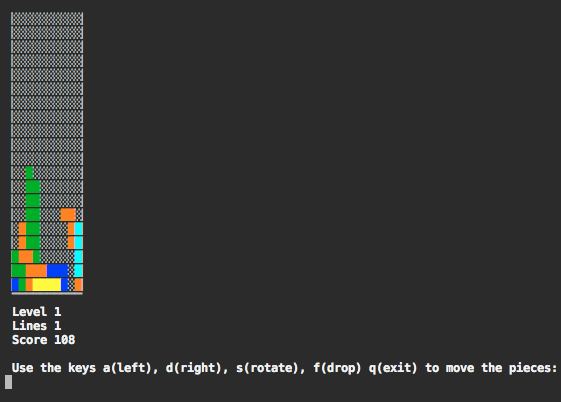
\includegraphics[scale=0.7]{resources/img/game}
	\label{use-cases}
\end{center}

\subsection{List of Requirements}
\label{sec:requirements}
\begin{table}[H]
	\centering
	%\caption{My caption}
	\label{tab:list-of-requirements}
	\begin{tabular}{|l|l|p{9cm}|}
		\hline
		\textbf{Id} & \textbf{Priority} & \textbf{Description} \\ \hline
		R1 & Mandatory         & The player can view his score and level \\ \hline
		R2 & Mandatory         & The game allows five movements - rotation, left, right, down and drop \\ \hline
		R3 & Opcional         & The player should be able to leave the game when he wants \\ \hline
		R4 & Mandatory         & The player has access to a footnote where the rules to play the game are displayed \\ \hline
		R5 & Mandatory         & The tetraminoes are spawned in a random order to be played\\ \hline
		R6 & Mandatory         & When one or more rows are full of blocks they must be cleared \\ \hline
		R7 & Mandatory         & If tetraminoes surpass the skyline the game is over \\ \hline
		R8 & Opcional          & Time to time the level advances and the game becomes more difficult \\ \hline
		R9 & Mandatory        & Each tetramino is formed by four squares named minoes \\ \hline
	\end{tabular}
\end{table}

These requirements are directly translated onto use cases as shown next.
\section{Visual UML Model} 


\subsection{Use Case Model}

In all use cases we have made an assumption that all keyboard game keys are functioning properly.

\begin{center}
	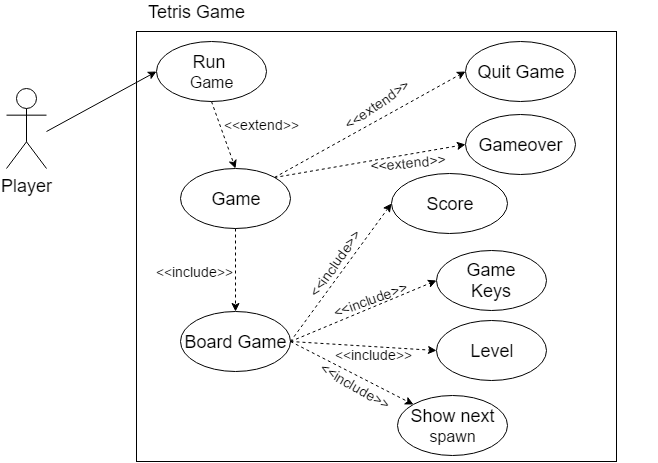
\includegraphics[scale=0.55]{resources/img/use_cases1}
	\label{use-cases}
\end{center}

\begin{center}
	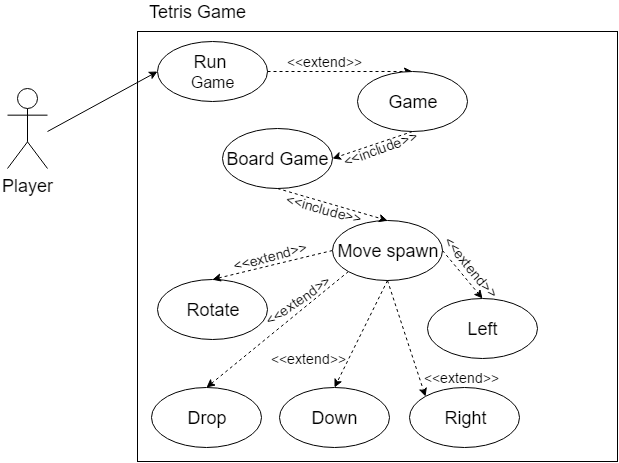
\includegraphics[scale=0.55]{resources/img/use_cases2}
\end{center}

The main use cases are described below: 

\begin{table}[H]
	\centering
	%	\caption{Use case board}
	\label{use-case-board}
	\begin{tabular}{|l| p{9cm}|}
		\hline
		\textbf{Scenario}        & \textbf{View Board Game} \\ \hline
		\textbf{Description}     &  The player can see his actual  difficulty level, score, keys to play the game and the next spawn\\ \hline
		\textbf{Pre-conditions}  & 	
		\begin{tabular}[c]{@{}l@{}}
			The game is running
		\end{tabular}  \\ \hline
		\textbf{Post-conditions} &  The player can view the information updated according to his performance during the game \\ \hline
		\textbf{Steps}           &  (none) \\ \hline
		\textbf{Exceptions}      &  (none) \\ \hline
	\end{tabular}
\end{table}

\begin{table}[H]
	\centering
	%	\caption{Use case gameover}
	\label{use-case-gameover}
	\begin{tabular}{|l| p{9cm}|}
		\hline
		\textbf{Scenario}        & \textbf{Gameover} \\ \hline
		\textbf{Description}     &  The player will finish the game \\ \hline
		\textbf{Pre-conditions}  & 	
		\begin{tabular}[c]{@{}l@{}}
			The game is running
		\end{tabular}  \\ \hline
		\textbf{Post-conditions} &  Game will reach the end and close \\ \hline
		\textbf{Steps}           &  \begin{enumerate}
			\item Play the game pressing the right keys
			\item Update score and level
			\item The game will eventually reach the end - gameover
		\end{enumerate} \\ \hline
		\textbf{Exceptions}      &  (none) \\ \hline
	\end{tabular}
\end{table}

\begin{table}[H]
	\centering
%	\caption{Use case rotation}
	\label{use-case-rotation}
	\begin{tabular}{|l| p{9cm}|}
		\hline
		\textbf{Scenario}        & \textbf{Rotation Move} \\ \hline
		\textbf{Description}     &  Rotate a tetramino when is falling \\ \hline
		\textbf{Pre-conditions}  & 	
			\begin{tabular}[c]{@{}l@{}}
				 Tetramino must not be frozen in place
			 \end{tabular}  \\ \hline
		\textbf{Post-conditions} &  Tetramino position has changed  \\ \hline
		\textbf{Steps}           &  The player must click on a key that allows rotation  \\ \hline
		\textbf{Exceptions}      &  When, simultaneously, try to rotate and the spawn reached one final position or the skyline pf the board \\ \hline
	\end{tabular}
\end{table}

\begin{table}[H]
	\centering
	%	\caption{Use case drop}
	\label{use-case-drop}
	\begin{tabular}{|l| p{9cm}|}
		\hline
		\textbf{Scenario}        & \textbf{Drop Move} \\ \hline
		\textbf{Description}     &  Accelerates the tetramino falling and position it as it was before reach the final position \\ \hline
		\textbf{Pre-conditions}  & 	
		\begin{tabular}[c]{@{}l@{}}
			Tetramino must not be frozen in place
		\end{tabular}  \\ \hline
		\textbf{Post-conditions} &  Tetramino position has changed  \\ \hline
		\textbf{Steps}           &  The player must click on a key that allows falling spawn  \\ \hline
		\textbf{Exceptions}      &  (none) \\ \hline
	\end{tabular}
\end{table}

\subsection{Class Model}
\begin{table}[H]
	\centering
	\label{description-classes}
	\begin{tabular}{|l|p{8cm}|}
	\hline
	\textbf{Class} 			   & \textbf{Description}	\\	\hline
	Game		   			   &	Core model; defines the state variables and operations available to the players	\\	\hline
	Board		   			   &	Defines a game environment for playing and where each piece of tetraminoes can stay \\	\hline
	Tetramino	   			   &	Defines one general piece to play with	\\	\hline
	TetraminoI/J/L/O/S/T/Z	   &	Defines one specific piece and is a subclass of Tetramino \\	\hline
	TestCaseExtra  			   &	Superclass for test classes; defines assertEquals and assertTrue	\\	\hline
	TestTetris	   			   &	Defines the test/usage scenarios and test cases for the tetris game	\\	\hline
	\end{tabular}
	\caption{Description of each class}
\end{table}
\newgeometry{left=2.2cm,top=2cm,bottom=2cm}
\begin{center}
	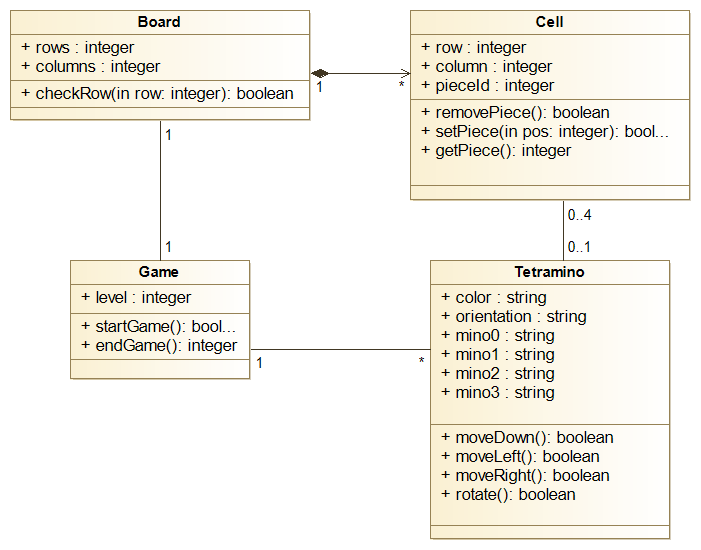
\includegraphics[scale=0.55]{resources/img/uml}
	\label{uml}
\end{center}
\restoregeometry

\section{Formal VDM++ Model}

\subsection{Game}
\begin{vdmpp}[breaklines=true]
class Game

 -- Represents the whole game, and provides all the necessary
 -- operations for playing it.
 
 
 types
 
  public String = seq of char;


 instance variables
  
  -- The game board.
  private board  : Board;
  -- The current game tetramino.
  private tetramino : Tetramino;
  -- Indicates if the game is finished.
  private gameOver : bool   := false; 
  -- The game score. 
  private score  : nat   := 0;
  -- The number of completed lines in the game.
  private lines  : nat   := 0;
  -- The level of the game. 
  private level  : nat1   := 1;
  
  -- The scores that lines make, according to the number of lines 
  -- made at once (1, 2, 3 or 4).
  private static lineScores : seq of nat
   := [100, 300, 400, 800];
  
  
 operations
 
(*@
\label{Game:35}
@*)
  public Game : () ==> Game
  Game() ==
   board := new Board();
    
(*@
\label{getBoard:39}
@*)
    public getBoard: () ==> Board
    getBoard() ==
     return board;
        
(*@
\label{setGameOver:43}
@*)
  public setGameOver : () ==> ()
  setGameOver() ==
   gameOver := true;
   
(*@
\label{getGameOver:47}
@*)
  public getGameOver : () ==> bool
  getGameOver() ==
   return gameOver;
       
    -- Generates a new tetramino of the specified type.
(*@
\label{newTetramino:52}
@*)
  public newTetramino : nat1 ==> ()
  newTetramino(id) == (  
   cases id:
    1 -> tetramino := new TetraminoI(self),
    2 -> tetramino := new TetraminoJ(self),
    3 -> tetramino := new TetraminoL(self),
    4 -> tetramino := new TetraminoO(self),
    5 -> tetramino := new TetraminoS(self),
    6 -> tetramino := new TetraminoT(self),
    7 -> tetramino := new TetraminoZ(self)
   end;
  )
  pre id >= 1 and id <= 7;
  
    -- Generates a new random tetramino.
(*@
\label{newRandomTetramino:67}
@*)
  public newRandomTetramino: () ==> ()
  newRandomTetramino() == 
   newTetramino(MATH`rand(7) + 1);
  
    -- Tries to move the current tetramino down.
(*@
\label{down:72}
@*)
  public down : () ==> bool
  down() ==
   return tetramino.moveDown(board);
   
    -- Tries to move the current tetramino left.
(*@
\label{left:77}
@*)
  public left : () ==> bool
  left() ==
   return tetramino.moveLeft(board);

    -- Tries to move the current tetramino right.
(*@
\label{right:82}
@*)
  public right : () ==> bool
  right() ==
   return tetramino.moveRight(board);
   
    -- Tries to rotate the current tetramino.
(*@
\label{rotate:87}
@*)
  public rotate : () ==> bool
  rotate() ==
   return tetramino.rotate(board);

    -- Drops the current tetramino to the bottom of the board. 
    -- Also updates the score, using the current level and the
    -- total distance of the drop. 
(*@
\label{drop:94}
@*)
  public drop : () ==> nat
  drop() == (
   dcl dropDistance: nat := tetramino.drop(board);
   score := score + dropDistance * level;
   return dropDistance;
  );
  
  -- Checks all game lines for completion and updates the game
  -- score according to the number of completed lines and the
  -- current game level.
(*@
\label{checkLines:104}
@*)
  public checkLines : () ==> nat
  checkLines() == (
   dcl newLines: nat := board.checkRows();
   lines := lines + newLines;
   if newLines > 0 then score := score + lineScores(newLines) * level;
   level := 1 + (lines div 10);
   return newLines
  );

(*@
\label{getScore:113}
@*)
  public getScore : () ==> nat
  getScore() == return score;
   
(*@
\label{getLines:116}
@*)
  public getLines : () ==> nat
  getLines() == return lines;

(*@
\label{getLevel:119}
@*)
  public getLevel : () ==> nat1
  getLevel() == return level;
  
  -- Returns a printing string of the board.
  -- If blackConsole is true, there are only three strings
  -- possible, depending on whether the position is empty or filled
  -- and diferentiating the invisible lines.
  -- If blackConsole is false, each tetramino will have a different
  -- print, according to its color.
(*@
\label{printBoard:128}
@*)
  public printBoard : bool * bool * bool ==> String
  printBoard(printNow, blackConsole, testPrint) == 
   return board.getBoardPrint(printNow, blackConsole, testPrint);
   
end Game
\end{vdmpp}

\subsection{Board}
\begin{vdmpp}[breaklines=true]
class Board

 -- Represents the game board, with its matrix.


 types
  
  -- Position in the board.
  public Position = seq of int
  -- A position is a sequence with exactly to integers.
  inv position == len position = 2;
  -- The board matrix is represented by a map.
  public Matrix = map Position to nat;


 instance variables
 
  -- Total number of rows in the board, including two lines that
  -- are not displayed for the user to see.
  public static maxRow  : nat1   := 22;
  -- Total number of rows that are visible during gameplay.
  public static maxVisibleRow : nat1   := 20;
  -- Total number of columns in the board.
  public static maxColumn  : nat1   := 10;

  -- Aids for printing the board matrix in the console.
  private print_startTag  : Game`String := "|";
  private print_endTag  : Game`String := "|\n";
  private print_bottomLine : Game`String := " ----------";
                                       
  -- The matrix attributes to each position in the board
  -- a natural number: 0 if the position is empty; the id of the
  -- tetramino if it is occupied.
  private matrix     : Matrix  := {|->};
     
                                                      
 operations
 
  public Board : () ==> Board
(*@
\label{Board:40}
@*)
  Board() == ( 
   initBoard();
  );
  
  -- Initiates the board matrix with all positions empty,
  -- that is, with zeros.
  private initBoard : () ==> ()
(*@
\label{initBoard:47}
@*)
  initBoard() == (  
   for i = 1 to maxRow do
    for j = 1 to maxColumn do
     matrix := matrix ++ {[i,j] |-> 0}
  )
  post matrix([1,1]) = 0 and matrix([maxRow, maxColumn]) = 0;

  -- Returns a string containing the board matrix in its
  -- printing form. If the boolean printNow is true, the matrix is
  -- immediately printed. If the boolean blackConsole is true, the
  -- matrix is printed without using colors. If the boolean testPrint
  -- is true, the invisible lines are printed for test purposes.
  public getBoardPrint : bool * bool * bool ==> Game`String
(*@
\label{getBoardPrint:60}
@*)
  getBoardPrint(printNow, blackConsole, testPrint) == ( 
   dcl print_board : Game`String := "\n";
   dcl start_row : nat1 := 3;
   if testPrint then start_row := 1;   
   for i = start_row to maxRow do(
    print_board := print_board ^ print_startTag;
      for j=1 to maxColumn do
       print_board := print_board 
        ^ getCellPrint(matrix([i,j]), i, blackConsole);
      print_board := print_board ^  print_endTag;
     );
     if printNow then
      IO`println(print_board ^ print_bottomLine);
    return print_board ^ print_bottomLine ;                   
  );
  
  -- Returns the string corresponding to a board cell print.
  -- If blackConsole is true, there are only three strings
  -- possible, depending on whether the position is empty or filled
  -- and diferentiating the invisible lines.
  -- If blackConsole is false, each tetramino will have a different
  -- print, according to its color.
  private getCellPrint: nat * nat * bool ==> Game`String
(*@
\label{getCellPrint:83}
@*)
  getCellPrint(id, row, blackConsole) == (
   if blackConsole then
    cases id:
     0 -> if row < 3 then return " " else return "#",
     others -> return "*"
    end
   else
    cases id:
     0 -> if row < 3 then return " " else return "#",
     1 -> return "\u001B[38;5;51m" ^ "*" ^ "\u001B[0m",
     2 -> return "\u001B[38;5;21m" ^ "*" ^ "\u001B[0m",
     3 -> return "\u001B[38;5;208m" ^ "*" ^ "\u001B[0m",
     4 -> return "\u001B[38;5;226m" ^ "*" ^ "\u001B[0m",
     5 -> return "\u001B[38;5;34m" ^ "*" ^ "\u001B[0m",
     6 -> return "\u001B[38;5;165m" ^ "*" ^ "\u001B[0m",
     others -> return "\u001B[38;5;196m" ^ "*" ^ "\u001B[0m"    
    end
  );
  
  -- Checks a board row to determine if it is completely filled
  -- with tetramino cells. In affirmative case, the row is removed
  -- from the board and the rows above it are shifted down.
  private checkRow : int ==> bool
(*@
\label{checkRow:106}
@*)
  checkRow(row) == (
   for column = 1 to maxColumn do
    if (matrix([row, column]) = 0) then return false;
   for i = row - 1 to 1 by -1 do
    for j = 1 to maxColumn do
     matrix([i + 1, j]) := matrix([i, j]);
   return true
  )
  pre row >= 1 and row <= maxRow;
  
  -- Checks all the rows of the board and returns the number of rows
  -- that where removed.
  public checkRows : () ==> nat
(*@
\label{checkRows:119}
@*)
  checkRows() == (
   dcl result : nat := 0;
   for row = 1 to maxRow do
    if checkRow(row) then result := result + 1;
   return result
  )
  post RESULT <= maxRow;
  
  public setMatrixPosition : Position * nat ==> ()
(*@
\label{setMatrixPosition:128}
@*)
  setMatrixPosition(position, value) ==
   matrix(position) := value
  pre Tetramino`checkPosition(position, 1, maxRow, 1, maxColumn);
  
  public getMatrixPosition : Position ==> nat
(*@
\label{getMatrixPosition:133}
@*)
  getMatrixPosition(position) ==
   return matrix(position)  
  pre Tetramino`checkPosition(position, 1, maxRow, 1, maxColumn);
 
end Board
\end{vdmpp}

\subsection{Tetramino}
\begin{vdmpp}[breaklines=true]
class Tetramino

 -- Defines a tetris piece, with all its relevant attributes.
 -- The position of the tetramino is represented by the position of 
 -- its minoes, which are the four cells composing the tetramino.


 types

  public Color = <Cyan> | <Blue> | <Orange> 
   | <Yellow> | <Green> | <Purple> | <Red>;
  public Minoes = seq of Board`Position
  -- There are always 4 minoes in each tetramino.
  inv minoes == len minoes = 4 


 instance variables
 
  -- Color of the piece, to aid in visualization
  private color  : Color  := <Cyan>;
  -- Id of the piece, to simplify its representation in the board
  private id   : nat1   := 1;
  -- The current orientation of the tetramino, since it can rotate
  private orientation : nat   := 0;
  -- The positions of each of the individual cells of the tetramino
  private minoes  : Minoes := [[1, 1], [1, 2], [1, 3], [1, 4]];
 
  -- The id is a natural number between 1 and 7,
  -- because there are 7 different types of tetraminoes
  -- The orientation is a number between 0 and 3,
  -- because there are at most 4 different orientations,
  -- depending on the tetramino type.
  inv id <= 7 and orientation < 4
  
 
 functions
 
  -- Checks if a given position is contained within the expected parameters.
(*@
\label{checkPosition:39}
@*)
  public checkPosition : Board`Position * int * int * int * int -> bool
  checkPosition(position, min1, max1, min2, max2) == 
   position(1) >= min1
   and position(1) <= max1 
   and position(2) >= min2
   and position(2) <= max2;
  
  -- Checks that all the tetramino cells have different positions,
  -- and that those positions are inside the expected parameters,
  -- which will be the board limits 
(*@
\label{checkMinoes:49}
@*)
  public checkMinoes: Minoes * int * int * int * int -> bool
  checkMinoes(minoes, min1, max1, min2, max2) ==
   card elems minoes = 4 
   and forall mino in set elems minoes & 
    checkPosition(mino, min1, max1, min2, max2)
 
 
 operations
  
(*@
\label{setColor:58}
@*)
  protected setColor : Color ==> ()
  setColor(c) == color := c;
  
(*@
\label{setId:61}
@*)
  protected setId : nat ==> ()
  setId(i) == id := i
  pre i >= 1 and i <= 7;
  
(*@
\label{getOrientation:65}
@*)
  public getOrientation : () ==> nat
  getOrientation() == return orientation
  post RESULT < 4;

  -- Given the position of the first of the four minoes, this operation
  -- sets the position of remaining three minoes. It also places the tetramino
  -- on the board if all positions are valid, otherwise, the tetramino remains
  -- in its original position.
(*@
\label{setMinoes:73}
@*)
  private setMinoes : Board * Board`Position ==> bool
  setMinoes(board, position) == (
   dcl tempMinoes : Minoes := minoes;
   dcl tempPosition : Board`Position := position;
   removeTetramino(board);
   for i = 1 to 4 do (
    if (validPosition(board, tempPosition)) 
    then tempMinoes(i) := tempPosition
    else (
     addTetramino(board);
     return false
    );
    tempPosition := getNextMino(tempPosition, i);
   );    
   minoes := tempMinoes;
   addTetramino(board);
   return true
  )
  pre checkPosition(position, -1, Board`maxRow + 2, -1, Board`maxColumn + 2)
  post checkMinoes(minoes, 1, Board`maxRow, 1, Board`maxColumn);
  
  -- Very similar to the previous operation, but this one is used only when a 
  -- tetramino is generated. It does not remove the tetramino from its previous
  -- position on the board (since it was never placed) and if at least one of the
  -- positions of the minoes is invalid, it declares the game over.
(*@
\label{initialSetMinoes:98}
@*)
  protected initialSetMinoes : Game * Board`Position ==> ()
  initialSetMinoes(game, position) == (
   dcl tempPosition : Board`Position := position;
   dcl tempMinoes : Minoes := minoes;
   for i = 1 to 4 do (
    if (validPosition(game.getBoard(), tempPosition)) 
    then (
     tempMinoes(i) := tempPosition;
     tempPosition := getNextMino(tempPosition, i)
    ) 
    else game.setGameOver()
   );   
   if not game.getGameOver() then (
    minoes := tempMinoes;
    addTetramino(game.getBoard())
   )
  )
  pre checkPosition(position, 1, Board`maxRow, 1, Board`maxColumn)
  post checkMinoes(minoes, 1, Board`maxRow, 1, Board`maxColumn);
  
  -- Given the position of one mino it computes the position of the next mino
  -- in the tetramino. The current mino is identified by its index within the
  -- tetramino. This is highly dependent on the type of tetramino, so can 
  -- only be defined in each subclass.
(*@
\label{getNextMino:122}
@*)
  protected getNextMino: Board`Position * nat ==> Board`Position
  getNextMino(position, index) ==
   is subclass responsibility;
   
  -- Given the current position of the first mino of a tetramino, determines
  -- the position of that mino after the tetramino is rotated.
(*@
\label{getRotatedMino:128}
@*)
  protected getRotatedMino: Board`Position ==> Board`Position
  getRotatedMino(position) ==
   is subclass responsibility;

  -- Checks if a given position on the board is valid for occupation, that is, 
  -- if it is inside the board limits and not currently occupied by some mino
(*@
\label{validPosition:134}
@*)
  protected validPosition : Board * Board`Position ==> bool
  validPosition(board, position) == 
   return checkPosition(position, 1, Board`maxRow, 1, Board`maxColumn) 
    and board.getMatrixPosition(position) = 0;

  -- Removes the tetramino from the board.
(*@
\label{removeTetramino:140}
@*)
  protected removeTetramino : Board ==> ()
  removeTetramino(board) ==
   for mino in minoes do
    board.setMatrixPosition(mino, 0)
  pre checkMinoes(minoes, 1, Board`maxRow, 1, Board`maxColumn);

  -- Places the tetramino in the board.
(*@
\label{addTetramino:147}
@*)
  protected addTetramino : Board ==> ()
  addTetramino(board) ==
   for mino in minoes do
    board.setMatrixPosition(mino, id)
  pre checkMinoes(minoes, 1, Board`maxRow, 1, Board`maxColumn);

  -- Moves the tetramino down in the board.
(*@
\label{moveDown:154}
@*)
  public moveDown : Board ==> bool
  moveDown(board) == 
   return setMinoes(board, [minoes(1)(1) + 1, minoes(1)(2)])
  pre checkMinoes(minoes, 1, Board`maxRow, 1, Board`maxColumn)
  post checkMinoes(minoes, 1, Board`maxRow, 1, Board`maxColumn);
     
  -- Moves the tetramino left in the board.
(*@
\label{moveLeft:161}
@*)
  public moveLeft : Board ==> bool
  moveLeft(board) == 
   return setMinoes(board, [minoes(1)(1), minoes(1)(2) - 1])
  pre checkMinoes(minoes, 1, Board`maxRow, 1, Board`maxColumn)
  post checkMinoes(minoes, 1, Board`maxRow, 1, Board`maxColumn);
  
  -- Moves the tetramino right in the board.
(*@
\label{moveRight:168}
@*)
  public moveRight : Board ==> bool
  moveRight(board) == 
   return setMinoes(board, [minoes(1)(1), minoes(1)(2) + 1])
  pre checkMinoes(minoes, 1, Board`maxRow, 1, Board`maxColumn)
  post checkMinoes(minoes, 1, Board`maxRow, 1, Board`maxColumn);

  -- Rotates the tetramino in the board.
(*@
\label{rotate:175}
@*)
  public rotate : Board ==> bool
  rotate(board) == (
   dcl position : Board`Position := getRotatedMino(minoes(1));
   orientation := (orientation + 1) mod 4;
   return setMinoes(board, position)
  )
  pre checkMinoes(minoes, 1, Board`maxRow, 1, Board`maxColumn)
  post checkMinoes(minoes, 1, Board`maxRow, 1, Board`maxColumn);
  
  -- Drops the tetramino to the lowest available position in the board.
(*@
\label{drop:185}
@*)
  public drop : Board ==> nat
  drop(board) == (
   dcl result : nat := 0;
   while moveDown(board) do 
    result := result + 1;
   return result
  )
  pre checkMinoes(minoes, 1, Board`maxRow, 1, Board`maxColumn)
  post checkMinoes(minoes, 1, Board`maxRow, 1, Board`maxColumn) 
   and RESULT < Board`maxRow;
  
end Tetramino
\end{vdmpp}
\bigskip
\begin{longtable}{|l|r|r|r|}
\hline
Function or operation & Line & Coverage & Calls \\
\hline
\hline
\hyperref[addTetramino:147]{addTetramino} & 147&100.0\% & 1646 \\
\hline
\hyperref[checkMinoes:49]{checkMinoes} & 49&100.0\% & 8172 \\
\hline
\hyperref[checkPosition:39]{checkPosition} & 39&100.0\% & 145640 \\
\hline
\hyperref[drop:185]{drop} & 185&100.0\% & 62 \\
\hline
\hyperref[getNextMino:122]{getNextMino} & 122&100.0\% & 2 \\
\hline
\hyperref[getOrientation:65]{getOrientation} & 65&100.0\% & 6392 \\
\hline
\hyperref[getRotatedMino:128]{getRotatedMino} & 128&100.0\% & 2 \\
\hline
\hyperref[initialSetMinoes:98]{initialSetMinoes} & 98&100.0\% & 62 \\
\hline
\hyperref[moveDown:154]{moveDown} & 154&100.0\% & 1077 \\
\hline
\hyperref[moveLeft:161]{moveLeft} & 161&100.0\% & 248 \\
\hline
\hyperref[moveRight:168]{moveRight} & 168&100.0\% & 190 \\
\hline
\hyperref[removeTetramino:140]{removeTetramino} & 140&100.0\% & 1585 \\
\hline
\hyperref[rotate:175]{rotate} & 175&100.0\% & 70 \\
\hline
\hyperref[setColor:58]{setColor} & 58&100.0\% & 62 \\
\hline
\hyperref[setId:61]{setId} & 61&100.0\% & 62 \\
\hline
\hyperref[setMinoes:73]{setMinoes} & 73&100.0\% & 1585 \\
\hline
\hyperref[validPosition:134]{validPosition} & 134&100.0\% & 6428 \\
\hline
\hline
Tetramino.vdmpp & & 100.0\% & 173285 \\
\hline
\end{longtable}


\subsection{TetraminoI}
\begin{vdmpp}[breaklines=true]
class TetraminoI is subclass of Tetramino

 -- Tetramino of the type I: xxxx
 -- 
 --
 -- Minoes:         1234
 -- 
 
  
 operations
 
  public TetraminoI : Game ==> TetraminoI
(*@
\label{TetraminoI:13}
@*)
  TetraminoI(game) == (
   Tetramino`setColor(<Cyan>);
   Tetramino`setId(1);
   Tetramino`initialSetMinoes(game, [2, 4]);
   return self
  );
  
  protected getNextMino: Board`Position * nat ==> Board`Position
(*@
\label{getNextMino:21}
@*)
  getNextMino(position, index) == (
   dcl result : Board`Position := position;
   cases Tetramino`getOrientation():
    0 -> result(2) := position(2) + 1,
    1 -> result(1) := position(1) + 1,
    2 -> result(2) := position(2) - 1,
    3 -> result(1) := position(1) - 1
   end;
   return result
  )
  pre Tetramino`checkPosition(position, 1, Board`maxRow, 1, Board`maxColumn)
  post Tetramino`checkPosition(RESULT, 0, Board`maxRow + 1, 0, Board`maxColumn + 1);
  
  protected getRotatedMino: Board`Position ==> Board`Position
(*@
\label{getRotatedMino:35}
@*)
  getRotatedMino(position) == (
   dcl result : Board`Position := position;
   cases Tetramino`getOrientation():
    0 -> (
     result(1) := position(1) - 1; 
     result(2) := position(2) + 2;
     ),
    1 -> (
     result(1) := position(1) + 2; 
     result(2) := position(2) + 1;
     ),
    2 -> (
     result(1) := position(1) + 1; 
     result(2) := position(2) - 2;
     ),
    3 -> (
     result(1) := position(1) - 2; 
     result(2) := position(2) - 1;
     )
   end;
   return result
  )
  pre Tetramino`checkPosition(position, 1, Board`maxRow, 1, Board`maxColumn)
  post Tetramino`checkPosition(RESULT, -1, Board`maxRow + 2, -1, Board`maxColumn + 2); 
  
      
end TetraminoI
\end{vdmpp}

\subsection{TetraminoJ}
\begin{vdmpp}[breaklines=true]
class TetraminoJ is subclass of Tetramino
  
 -- Tetramino of the type J: x
 --       xxx
 -- 
 -- Minoes:       1
 --        234

 
 operations
 
  public TetraminoJ : (Game) ==> TetraminoJ
  TetraminoJ(game) == (
   Tetramino`setColor(<Blue>);
(*@
\label{TetraminoJ:15}
@*)
   Tetramino`setId(2);
   Tetramino`initialSetMinoes(game, [1, 4]);
   return self
  );

  protected getNextMino: Board`Position * nat ==> Board`Position
  getNextMino(position, index) == (
   dcl result : Board`Position := position;
(*@
\label{getNextMino:23}
@*)
   cases Tetramino`getOrientation():
    0 -> (
     cases index:
      1 -> result(1) := position(1) + 1,
      others -> result(2) := position(2) + 1
     end
    ),
    1 -> (
     cases index:
      1 -> result(2) := position(2) - 1,
      others -> result(1) := position(1) + 1
     end
    ),
    2 -> (
     cases index:
      1 -> result(1) := position(1) - 1,
      others -> result(2) := position(2) - 1
     end
    ),
    3 -> (
     cases index:
      1 -> result(2) := position(2) + 1,
      others -> result(1) := position(1) - 1
     end
    )
   end;
   return result
  )
  pre index in set {1, ..., 4} 
   and Tetramino`checkPosition(position, 1, Board`maxRow, 1, Board`maxColumn)
  post Tetramino`checkPosition(RESULT, 0, Board`maxRow + 1, 0, Board`maxColumn + 1);

  protected getRotatedMino: Board`Position ==> Board`Position
  getRotatedMino(position) == (
   dcl result : Board`Position := position;
(*@
\label{getRotatedMino:58}
@*)
   cases Tetramino`getOrientation():
    0 -> result(2) := position(2) + 2,
    1 -> result(1) := position(1) + 2,
    2 -> result(2) := position(2) - 2,
    3 -> result(1) := position(1) - 2
   end;
   return result
  )
  pre Tetramino`checkPosition(position, 1, Board`maxRow, 1, Board`maxColumn)
  post Tetramino`checkPosition(RESULT, -1, Board`maxRow + 2, -1, Board`maxColumn + 2);

end TetraminoJ
\end{vdmpp}

\subsection{TetraminoL}
\begin{vdmpp}[breaklines=true]
class TetraminoL is subclass of Tetramino
  
 -- Tetramino of the type J: x
 --       xxx
 --
 -- Minoes:         1
 --        432


 operations
 
(*@
\label{TetraminoL:12}
@*)
  public TetraminoL : (Game) ==> TetraminoL
  TetraminoL(game) == (
   Tetramino`setColor(<Orange>);
   Tetramino`setId(3);
   Tetramino`initialSetMinoes(game, [1, 6]);
   return self
  );

(*@
\label{getNextMino:20}
@*)
  protected getNextMino: Board`Position * nat ==> Board`Position
  getNextMino(position, index) == (
   dcl result : Board`Position := position;
   cases Tetramino`getOrientation():
    0 -> (
     cases index:
      1 -> result(1) := position(1) + 1,
      others -> result(2) := position(2) - 1
     end
    ),
    1 -> (
     cases index:
      1 -> result(2) := position(2) - 1,
      others -> result(1) := position(1) - 1
     end
    ),
    2 -> (
     cases index:
      1 -> result(1) := position(1) - 1,
      others -> result(2) := position(2) + 1
     end
    ),
    3 -> (
     cases index:
      1 -> result(2) := position(2) + 1,
      others -> result(1) := position(1) + 1
     end
    )
   end;
   return result
  )
  pre index in set {1, ..., 4} 
   and Tetramino`checkPosition(position, 1, Board`maxRow, 1, Board`maxColumn)
  post Tetramino`checkPosition(RESULT, 0, Board`maxRow + 1, 0, Board`maxColumn + 1);
   
(*@
\label{getRotatedMino:55}
@*)
  protected getRotatedMino: Board`Position ==> Board`Position
  getRotatedMino(position) == (
   dcl result : Board`Position := position;
   cases Tetramino`getOrientation():
    0 -> result(1) := position(1) + 2,
    1 -> result(2) := position(2) - 2,
    2 -> result(1) := position(1) - 2,
    3 -> result(2) := position(2) + 2
   end;
   return result
  )
  pre Tetramino`checkPosition(position, 1, Board`maxRow, 1, Board`maxColumn)
  post Tetramino`checkPosition(RESULT, -1, Board`maxRow + 2, -1, Board`maxColumn + 2); 

end TetraminoL
\end{vdmpp}

\subsection{TetraminoO}
\begin{vdmpp}[breaklines=true]
class TetraminoO is subclass of Tetramino
  
 -- Tetramino of the type J: xx
 --         xx
 --  
 -- Minoes:       12
 --         43
 

 operations
(*@
\label{TetraminoO:11}
@*)
  public TetraminoO : (Game) ==> TetraminoO
  TetraminoO(game) == (
   Tetramino`setColor(<Yellow>);
   Tetramino`setId(4);
   Tetramino`initialSetMinoes(game, [1, 5]);
   return self
  );

(*@
\label{getNextMino:19}
@*)
  protected getNextMino: Board`Position * nat ==> Board`Position
  getNextMino(position, index) == (
   dcl result : Board`Position := position;
   cases Tetramino`getOrientation():
    0 -> (
     cases index:
      1 -> result(2) := position(2) + 1,
      2 -> result(1) := position(1) + 1,
      others -> result(2) := position(2) - 1
     end
    ),
    1 -> (
     cases index:
      1 -> result(1) := position(1) + 1,
      2 -> result(2) := position(2) - 1,
      others -> result(1) := position(1) - 1
     end
    ),
    2 -> (
     cases index:
      1 -> result(2) := position(2) - 1,
      2 -> result(1) := position(1) - 1,
      others -> result(2) := position(2) + 1
     end
    ),
    3 -> (
     cases index:
      1 -> result(1) := position(1) - 1,
      2 -> result(2) := position(2) + 1,
      others -> result(1) := position(1) + 1
     end
    )
   end;
   return result
  )
  pre index in set {1, ..., 4} 
   and Tetramino`checkPosition(position, 1, Board`maxRow, 1, Board`maxColumn)
  post Tetramino`checkPosition(RESULT, 0, Board`maxRow + 1, 0, Board`maxColumn + 1);
   
(*@
\label{getRotatedMino:58}
@*)
  protected getRotatedMino: Board`Position ==> Board`Position
  getRotatedMino(position) == (
   dcl result : Board`Position := position;
   cases Tetramino`getOrientation():
    0 -> result(2) := position(2) + 1,
    1 -> result(1) := position(1) + 1,
    2 -> result(2) := position(2) - 1,
    3 -> result(1) := position(1) - 1
   end;
   return result
  )
  pre Tetramino`checkPosition(position, 1, Board`maxRow, 1, Board`maxColumn)
  post Tetramino`checkPosition(RESULT, -1, Board`maxRow + 2, -1, Board`maxColumn + 2);

end TetraminoO
\end{vdmpp}

\subsection{TetraminoS}
\begin{vdmpp}[breaklines=true]
class TetraminoS is subclass of Tetramino
  
 -- Tetramino of the type J:  xx
 --        xx
 --
 -- Minoes:       21
 --        43
 
 
 operations
 
(*@
\label{TetraminoS:12}
@*)
  public TetraminoS : (Game) ==> TetraminoS
  TetraminoS(game) == (
   Tetramino`setColor(<Green>);
   Tetramino`setId(5);
   Tetramino`initialSetMinoes(game, [1, 6]);
   return self
  );
   
(*@
\label{getNextMino:20}
@*)
  protected getNextMino: Board`Position * nat ==> Board`Position
  getNextMino(position, index) == (
   dcl result : Board`Position := position;
   cases Tetramino`getOrientation():
    0 -> (
     cases index:
      2 -> result(1) := position(1) + 1,
      others -> result(2) := position(2) - 1
     end
    ),
    1 -> (
     cases index:
      2 -> result(2) := position(2) - 1,
      others -> result(1) := position(1) - 1
     end
    ),
    2 -> (
     cases index:
      2 -> result(1) := position(1) - 1,
      others -> result(2) := position(2) + 1
     end
    ),
    3 -> (
     cases index:
      2 -> result(2) := position(2) + 1,
      others -> result(1) := position(1) + 1
     end
    )
   end;
   return result
  )
  pre index in set {1, ..., 4} 
   and Tetramino`checkPosition(position, 1, Board`maxRow, 1, Board`maxColumn)
  post Tetramino`checkPosition(RESULT, 0, Board`maxRow + 1, 0, Board`maxColumn + 1);
   
(*@
\label{getRotatedMino:55}
@*)
  protected getRotatedMino: Board`Position ==> Board`Position
  getRotatedMino(position) == (
   dcl result : Board`Position := position;
   cases Tetramino`getOrientation():
    0 -> result(1) := position(1) + 2,
    1 -> result(2) := position(2) - 2,
    2 -> result(1) := position(1) - 2,
    3 -> result(2) := position(2) + 2
   end;
   return result
  )
  pre Tetramino`checkPosition(position, 1, Board`maxRow, 1, Board`maxColumn)
  post Tetramino`checkPosition(RESULT, -1, Board`maxRow + 2, -1, Board`maxColumn + 2);

end TetraminoS
\end{vdmpp}

\subsection{TetraminoT}
\begin{vdmpp}[breaklines=true]
class TetraminoT is subclass of Tetramino
  
 -- Tetramino of the type J:  x
 --       xxx
 --
 -- Minoes:        1
 --         234
 

 operations
 
(*@
\label{TetraminoT:12}
@*)
  public TetraminoT : (Game) ==> TetraminoT
  TetraminoT(game) == (
   Tetramino`setColor(<Purple>);
   Tetramino`setId(6);
   Tetramino`initialSetMinoes(game, [1, 5]);
   return self
  );

(*@
\label{getNextMino:20}
@*)
  protected getNextMino: Board`Position * nat ==> Board`Position
  getNextMino(position, index) == (
   dcl result : Board`Position := position;
   cases Tetramino`getOrientation():
    0 -> (
     cases index:
      1 -> (
       result(1) := position(1) + 1;
       result(2) := position(2) - 1;
      ),
      others -> result(2) := position(2) + 1
     end
    ),
    1 -> (
     cases index:
      1 -> (
       result(1) := position(1) - 1;
       result(2) := position(2) - 1;
      ),
      others -> result(1) := position(1) + 1
     end
    ),
    2 -> (
     cases index:
      1 -> (
       result(1) := position(1) - 1;
       result(2) := position(2) + 1;
      ),
      others -> result(2) := position(2) - 1
     end
    ),
    3 -> (
     cases index:
      1 -> (
       result(1) := position(1) + 1;
       result(2) := position(2) + 1;
      ),
      others -> result(1) := position(1) - 1
     end
    )
   end;
   return result
  )
  pre index in set {1, ..., 4} 
   and Tetramino`checkPosition(position, 1, Board`maxRow, 1, Board`maxColumn)
  post Tetramino`checkPosition(RESULT, 0, Board`maxRow + 1, 0, Board`maxColumn + 1);
  
(*@
\label{getRotatedMino:67}
@*)
  protected getRotatedMino: Board`Position ==> Board`Position
  getRotatedMino(position) == (
   dcl result : Board`Position := position;
   cases Tetramino`getOrientation():
    0 -> (
     result(1) := position(1) + 1; 
     result(2) := position(2) + 1;
     ),
    1 -> (
     result(1) := position(1) + 1; 
     result(2) := position(2) - 1;
     ),
    2 -> (
     result(1) := position(1) - 1; 
     result(2) := position(2) - 1;
     ),
    3 -> (
     result(1) := position(1) - 1; 
     result(2) := position(2) + 1;
     )
   end;
   return result
  )
  pre Tetramino`checkPosition(position, 1, Board`maxRow, 1, Board`maxColumn)
  post Tetramino`checkPosition(RESULT, -1, Board`maxRow + 2, -1, Board`maxColumn + 2);

end TetraminoT
\end{vdmpp}
\bigskip
\begin{longtable}{|l|r|r|r|}
\hline
Function or operation & Line & Coverage & Calls \\
\hline
\hline
\hyperref[TetraminoT:12]{TetraminoT} & 12&100.0\% & 2 \\
\hline
\hyperref[getNextMino:20]{getNextMino} & 20&100.0\% & 157 \\
\hline
\hyperref[getRotatedMino:67]{getRotatedMino} & 67&100.0\% & 5 \\
\hline
\hline
TetraminoT.vdmpp & & 100.0\% & 164 \\
\hline
\end{longtable}


\subsection{TetraminoZ}
\begin{vdmpp}[breaklines=true]
class TetraminoZ is subclass of Tetramino
  
 -- Tetramino of the type Z: xx
 --        xx
 --
 -- Minoes:      12
 --          34
 

 operations
 
(*@
\label{TetraminoZ:12}
@*)
  public TetraminoZ : (Game) ==> TetraminoZ
  TetraminoZ(game) == (
   Tetramino`setColor(<Red>);
   Tetramino`setId(7);
   Tetramino`initialSetMinoes(game, [1, 4]);
   return self
  );

(*@
\label{getNextMino:20}
@*)
  protected getNextMino: Board`Position * nat ==> Board`Position
  getNextMino(position, index) == (
   dcl result : Board`Position := position;
   cases Tetramino`getOrientation():
    0 -> (
     cases index:
      2 -> result(1) := position(1) + 1,
      others -> result(2) := position(2) + 1
     end
    ),
    1 -> (
     cases index:
      2 -> result(2) := position(2) - 1,
      others -> result(1) := position(1) + 1
     end
    ),
    2 -> (
     cases index:
      2 -> result(1) := position(1) - 1,
      others -> result(2) := position(2) - 1
     end
    ),
    3 -> (
     cases index:
      2 -> result(2) := position(2) + 1,
      others -> result(1) := position(1) - 1
     end
    )
   end;
   return result
  )
  pre index in set {1, ..., 4} 
   and Tetramino`checkPosition(position, 1, Board`maxRow, 1, Board`maxColumn)
  post Tetramino`checkPosition(RESULT, 0, Board`maxRow + 1, 0, Board`maxColumn + 1);
   
(*@
\label{getRotatedMino:55}
@*)
  protected getRotatedMino: Board`Position ==> Board`Position
  getRotatedMino(position) == (
   dcl result : Board`Position := position;
   cases Tetramino`getOrientation():
    0 -> result(2) := position(2) + 2,
    1 -> result(1) := position(1) + 2,
    2 -> result(2) := position(2) - 2,
    3 -> result(1) := position(1) - 2
   end;
   return result
  )
  pre Tetramino`checkPosition(position, 1, Board`maxRow, 1, Board`maxColumn)
  post Tetramino`checkPosition(RESULT, -1, Board`maxRow + 2, -1, Board`maxColumn + 2);

end TetraminoZ
\end{vdmpp}


\section{Model Validation}

We used test cases to validate our model, obtaining 100.0\% code coverage except in a very specific case, that is dully noted and justified. As exemplified in the Vending Machine code made available in the course page, we used assertions in our test cases, checking the board prints, the values and booleans obtained and the changes in game state.

\subsection{TestCaseExtra}
\begin{vdmpp}[breaklines=true]
class TestCaseExtra

 -- Class obtained from the Vending Machine example of MFES
 
 
 operations
 -- Simulates assertion checking by reducing it to pre-condition checking.
 -- If 'arg' does not hold, a pre-condition violation will be signaled.
(*@
\label{assertTrue:9}
@*)
 protected assertTrue: bool ==> ()
 assertTrue(arg) == 
  return 
 pre arg;
  
 -- Simulates assertion checking by reducing it to post-condition checking.
 -- If values are not equal, prints a message in the console and generates 
 -- a post-conditions violation.
(*@
\label{assertEqual:17}
@*)
 protected assertEqual: ? * ? ==> ()
 assertEqual(expected, actual) == 
  if expected <> actual then (*@\vdmnotcovered{(}@*)
     (*@\vdmnotcovered{IO`print}@*)((*@\vdmnotcovered{"Actual value ("}@*));
     (*@\vdmnotcovered{IO`print}@*)((*@\vdmnotcovered{actual}@*)); 
     (*@\vdmnotcovered{IO`print}@*)((*@\vdmnotcovered{") different from expected ("}@*));
     (*@\vdmnotcovered{IO`print}@*)((*@\vdmnotcovered{expected}@*));
     (*@\vdmnotcovered{IO`println}@*)((*@\vdmnotcovered{")\textbackslash n"}@*))
  )
 post expected = actual
 
end TestCaseExtra


\end{vdmpp}
\bigskip
\begin{longtable}{|l|r|r|r|}
\hline
Function or operation & Line & Coverage & Calls \\
\hline
\hline
\hyperref[assertEqual:17]{assertEqual} & 17&38.8\% & 121 \\
\hline
\hyperref[assertTrue:9]{assertTrue} & 9&100.0\% & 185 \\
\hline
\hline
TestCaseExtra.vdmpp & & 45.0\% & 306 \\
\hline
\end{longtable}


\subsection{TestTetris}
\begin{vdmpp}[breaklines=true]
class TestTetris is subclass of TestCaseExtra

 instance variables
 
  private printBoard : Game`String := "";
   

 operations
 
  -- Prints the initial board matrix and checks it is as should be for tests.
(*@
\label{initalMatrix:test:11}
@*)
  private initalMatrix_test: Game * bool * bool * bool ==> ()
  initalMatrix_test(game, printNow, blackConsole, testPrint) == (
   printBoard := game.printBoard(printNow, blackConsole, testPrint);
   assertEqual(printBoard, 
    "\n▕          ▏" ^
    "\n▕          ▏" ^
    "\n▕░░░░░░░░░░▏" ^
    "\n▕░░░░░░░░░░▏" ^
    "\n▕░░░░░░░░░░▏" ^
    "\n▕░░░░░░░░░░▏" ^
    "\n▕░░░░░░░░░░▏" ^
    "\n▕░░░░░░░░░░▏" ^
    "\n▕░░░░░░░░░░▏" ^
    "\n▕░░░░░░░░░░▏" ^
    "\n▕░░░░░░░░░░▏" ^
    "\n▕░░░░░░░░░░▏" ^
    "\n▕░░░░░░░░░░▏" ^
    "\n▕░░░░░░░░░░▏" ^
    "\n▕░░░░░░░░░░▏" ^
    "\n▕░░░░░░░░░░▏" ^
    "\n▕░░░░░░░░░░▏" ^
    "\n▕░░░░░░░░░░▏" ^
    "\n▕░░░░░░░░░░▏" ^
    "\n▕░░░░░░░░░░▏" ^
    "\n▕░░░░░░░░░░▏" ^
    "\n▕░░░░░░░░░░▏" ^
    "\n ▔▔▔▔▔▔▔▔▔▔")
  ); 

  -- Adds a tetramino of type I to the board and checks it is in the right position.
(*@
\label{addTetramino1:test:41}
@*)
  private addTetramino1_test: Game * bool * bool * bool ==> ()
  addTetramino1_test(game, printNow, blackConsole, testPrint) == (  
   game.newTetramino(1);
   printBoard := game.printBoard(printNow, blackConsole, testPrint);
   assertEqual(printBoard, 
    "\n▕          ▏" ^
    "\n▕   ████   ▏" ^
    "\n▕░░░░░░░░░░▏" ^
    "\n▕░░░░░░░░░░▏" ^
    "\n▕░░░░░░░░░░▏" ^
    "\n▕░░░░░░░░░░▏" ^
    "\n▕░░░░░░░░░░▏" ^
    "\n▕░░░░░░░░░░▏" ^
    "\n▕░░░░░░░░░░▏" ^
    "\n▕░░░░░░░░░░▏" ^
    "\n▕░░░░░░░░░░▏" ^
    "\n▕░░░░░░░░░░▏" ^
    "\n▕░░░░░░░░░░▏" ^
    "\n▕░░░░░░░░░░▏" ^
    "\n▕░░░░░░░░░░▏" ^
    "\n▕░░░░░░░░░░▏" ^
    "\n▕░░░░░░░░░░▏" ^
    "\n▕░░░░░░░░░░▏" ^
    "\n▕░░░░░░░░░░▏" ^
    "\n▕░░░░░░░░░░▏" ^
    "\n▕░░░░░░░░░░▏" ^
    "\n▕░░░░░░░░░░▏" ^
    "\n ▔▔▔▔▔▔▔▔▔▔")
  );

  -- Adds a tetramino of type J to the board and checks it is in the right position.
(*@
\label{addTetramino2:test:72}
@*)
  private addTetramino2_test: Game * bool * bool * bool ==> ()
  addTetramino2_test(game, printNow, blackConsole, testPrint) == (  
   game.newTetramino(2);
   printBoard := game.printBoard(printNow, blackConsole, testPrint);
   assertEqual(printBoard, 
    "\n▕   █      ▏" ^
    "\n▕   ███    ▏" ^
    "\n▕░░░░░░░░░░▏" ^
    "\n▕░░░░░░░░░░▏" ^
    "\n▕░░░░░░░░░░▏" ^
    "\n▕░░░░░░░░░░▏" ^
    "\n▕░░░░░░░░░░▏" ^
    "\n▕░░░░░░░░░░▏" ^
    "\n▕░░░░░░░░░░▏" ^
    "\n▕░░░░░░░░░░▏" ^
    "\n▕░░░░░░░░░░▏" ^
    "\n▕░░░░░░░░░░▏" ^
    "\n▕░░░░░░░░░░▏" ^
    "\n▕░░░░░░░░░░▏" ^
    "\n▕░░░░░░░░░░▏" ^
    "\n▕░░░░░░░░░░▏" ^
    "\n▕░░░░░░░░░░▏" ^
    "\n▕░░░░░░░░░░▏" ^
    "\n▕░░░░░░░░░░▏" ^
    "\n▕░░░░░░░░░░▏" ^
    "\n▕░░░░░░░░░░▏" ^
    "\n▕░░░████░░░▏" ^
    "\n ▔▔▔▔▔▔▔▔▔▔")
  );

  -- Adds a tetramino of type L to the board and checks it is in the right position.
(*@
\label{addTetramino3:test:103}
@*)
  private addTetramino3_test: Game * bool * bool * bool ==> ()
  addTetramino3_test(game, printNow, blackConsole, testPrint) == (  
   game.newTetramino(3);
   printBoard := game.printBoard(printNow, blackConsole, testPrint);
   assertEqual(printBoard, 
    "\n▕     █    ▏" ^
    "\n▕   ███    ▏" ^
    "\n▕░░░░░░░░░░▏" ^
    "\n▕░░░░░░░░░░▏" ^
    "\n▕░░░░░░░░░░▏" ^
    "\n▕░░░░░░░░░░▏" ^
    "\n▕░░░░░░░░░░▏" ^
    "\n▕░░░░░░░░░░▏" ^
    "\n▕░░░░░░░░░░▏" ^
    "\n▕░░░░░░░░░░▏" ^
    "\n▕░░░░░░░░░░▏" ^
    "\n▕░░░░░░░░░░▏" ^
    "\n▕░░░░░░░░░░▏" ^
    "\n▕░░░░░░░░░░▏" ^
    "\n▕░░░░░░░░░░▏" ^
    "\n▕░░░░░░░░░░▏" ^
    "\n▕░░░░░░░░░░▏" ^
    "\n▕░░░░░░░░░░▏" ^
    "\n▕░░░░░░░░░░▏" ^
    "\n▕░░░░░░░░░░▏" ^
    "\n▕█░░░░░░░░░▏" ^
    "\n▕███████░░░▏" ^
    "\n ▔▔▔▔▔▔▔▔▔▔")
  );

  -- Adds a tetramino of type O to the board and checks it is in the right position.
(*@
\label{addTetramino4:test:134}
@*)
  private addTetramino4_test: Game * bool * bool * bool ==> ()
  addTetramino4_test(game, printNow, blackConsole, testPrint) == (  
   game.newTetramino(4);
   printBoard := game.printBoard(printNow, blackConsole, testPrint);
   assertEqual(printBoard, 
    "\n▕    ██    ▏" ^
    "\n▕    ██    ▏" ^
    "\n▕░░░░░░░░░░▏" ^
    "\n▕░░░░░░░░░░▏" ^
    "\n▕░░░░░░░░░░▏" ^
    "\n▕░░░░░░░░░░▏" ^
    "\n▕░░░░░░░░░░▏" ^
    "\n▕░░░░░░░░░░▏" ^
    "\n▕░░░░░░░░░░▏" ^
    "\n▕░░░░░░░░░░▏" ^
    "\n▕░░░░░░░░░░▏" ^
    "\n▕░░░░░░░░░░▏" ^
    "\n▕░░░░░░░░░░▏" ^
    "\n▕░░░░░░░░░░▏" ^
    "\n▕░░░░░░░░░░▏" ^
    "\n▕░░░░░░░░░░▏" ^
    "\n▕░░░░░░░░░░▏" ^
    "\n▕░░░░░░░░░░▏" ^
    "\n▕░░░░░░░░░░▏" ^
    "\n▕░░░░░░░░░░▏" ^
    "\n▕░░░░░░░░░░▏" ^
    "\n▕█░░░░░░░░█▏" ^
    "\n ▔▔▔▔▔▔▔▔▔▔")
  );

  -- Adds a tetramino of type S to the board and checks it is in the right position.
(*@
\label{addTetramino5:test:165}
@*)
  private addTetramino5_test: Game * bool * bool * bool ==> ()
  addTetramino5_test(game, printNow, blackConsole, testPrint) == (  
   game.newTetramino(5);
   printBoard := game.printBoard(printNow, blackConsole, testPrint);
   assertEqual(printBoard, 
    "\n▕    ██    ▏" ^
    "\n▕   ██     ▏" ^
    "\n▕░░░░░░░░░░▏" ^
    "\n▕░░░░░░░░░░▏" ^
    "\n▕░░░░░░░░░░▏" ^
    "\n▕░░░░░░░░░░▏" ^
    "\n▕░░░░░░░░░░▏" ^
    "\n▕░░░░░░░░░░▏" ^
    "\n▕░░░░░░░░░░▏" ^
    "\n▕░░░░░░░░░░▏" ^
    "\n▕░░░░░░░░░░▏" ^
    "\n▕░░░░░░░░░░▏" ^
    "\n▕░░░░░░░░░░▏" ^
    "\n▕░░░░░░░░░░▏" ^
    "\n▕░░░░░░░░░░▏" ^
    "\n▕░░░░░░░░░░▏" ^
    "\n▕░░░░░░░░░░▏" ^
    "\n▕░░░░░░░░░░▏" ^
    "\n▕░░░░░░░░░░▏" ^
    "\n▕░░░░░░░░░░▏" ^
    "\n▕░░░░██░░░░▏" ^
    "\n▕█░░░██░░░█▏" ^
    "\n ▔▔▔▔▔▔▔▔▔▔")
  );

  -- Adds a tetramino of type T to the board and checks it is in the right position.
(*@
\label{addTetramino6:test:196}
@*)
  private addTetramino6_test: Game * bool * bool * bool ==> ()
  addTetramino6_test(game, printNow, blackConsole, testPrint) == (  
   game.newTetramino(6);
   printBoard := game.printBoard(printNow, blackConsole, testPrint);
   assertEqual(printBoard, 
    "\n▕    █     ▏" ^
    "\n▕   ███    ▏" ^
    "\n▕░░░░░░░░░░▏" ^
    "\n▕░░░░░░░░░░▏" ^
    "\n▕░░░░░░░░░░▏" ^
    "\n▕░░░░░░░░░░▏" ^
    "\n▕░░░░░░░░░░▏" ^
    "\n▕░░░░░░░░░░▏" ^
    "\n▕░░░░░░░░░░▏" ^
    "\n▕░░░░░░░░░░▏" ^
    "\n▕░░░░░░░░░░▏" ^
    "\n▕░░░░░░░░░░▏" ^
    "\n▕░░░░░░░░░░▏" ^
    "\n▕░░░░░░░░░░▏" ^
    "\n▕░░░░░░░░░░▏" ^
    "\n▕░░░░░░░░░░▏" ^
    "\n▕░░░░░░░░░░▏" ^
    "\n▕░░░░░░░░░░▏" ^
    "\n▕░░░░░░░░░░▏" ^
    "\n▕░░░░░░░░░░▏" ^
    "\n▕░░░░██░░██▏" ^
    "\n▕█░░░██░███▏" ^
    "\n ▔▔▔▔▔▔▔▔▔▔")
  );

  -- Adds a tetramino of type Z to the board and checks it is in the right position.
(*@
\label{addTetramino7:test:227}
@*)
  private addTetramino7_test: Game * bool * bool * bool ==> ()
  addTetramino7_test(game, printNow, blackConsole, testPrint) == (  
   game.newTetramino(7);
   printBoard := game.printBoard(printNow, blackConsole, testPrint);
   assertEqual(printBoard, 
    "\n▕   ██     ▏" ^
    "\n▕    ██    ▏" ^
    "\n▕░░░░░░░░░░▏" ^
    "\n▕░░░░░░░░░░▏" ^
    "\n▕░░░░░░░░░░▏" ^
    "\n▕░░░░░░░░░░▏" ^
    "\n▕░░░░░░░░░░▏" ^
    "\n▕░░░░░░░░░░▏" ^
    "\n▕░░░░░░░░░░▏" ^
    "\n▕░░░░░░░░░░▏" ^
    "\n▕░░░░░░░░░░▏" ^
    "\n▕░░░░░░░░░░▏" ^
    "\n▕░░░░░░░░░░▏" ^
    "\n▕░░░░░░░░░░▏" ^
    "\n▕░░░░░░░░░░▏" ^
    "\n▕░░░░░░░░░░▏" ^
    "\n▕░░░░░░░░░░▏" ^
    "\n▕░░░░░░░░░░▏" ^
    "\n▕░░░░░░░░░░▏" ^
    "\n▕░░░░░░█░░░▏" ^
    "\n▕░░░░██████▏" ^
    "\n▕█░░░██████▏" ^
    "\n ▔▔▔▔▔▔▔▔▔▔")
  );
  
  -- Adds another tetramino of type S to the board and checks it is in the right position.
(*@
\label{addTetramino8:test:258}
@*)
  private addTetramino8_test: Game * bool * bool * bool ==> ()
  addTetramino8_test(game, printNow, blackConsole, testPrint) == (  
   game.newTetramino(5);
   printBoard := game.printBoard(printNow, blackConsole, testPrint);
   assertEqual(printBoard, 
    "\n▕    ██    ▏" ^
    "\n▕   ██     ▏" ^
    "\n▕░░░░░░░░░░▏" ^
    "\n▕░░░░░░░░░░▏" ^
    "\n▕░░░░░░░░░░▏" ^
    "\n▕░░░░░░░░░░▏" ^
    "\n▕░░░░░░░░░░▏" ^
    "\n▕░░░░░░░░░░▏" ^
    "\n▕░░░░░░░░░░▏" ^
    "\n▕░░░░░░░░░░▏" ^
    "\n▕░░░░░░░░░░▏" ^
    "\n▕░░░░░░░░░░▏" ^
    "\n▕░░░░░░░░░░▏" ^
    "\n▕░░░░░░░░░░▏" ^
    "\n▕░░░░░░░░░░▏" ^
    "\n▕░░░░░░░░░░▏" ^
    "\n▕░░░░░░░░░░▏" ^
    "\n▕░░░░░░░░░░▏" ^
    "\n▕░░░░░░░░░░▏" ^
    "\n▕░░░░░░█░░░▏" ^
    "\n▕██░░██████▏" ^
    "\n▕███░██████▏" ^
    "\n ▔▔▔▔▔▔▔▔▔▔")
  );
  
  -- Moves the first tetramino several times and in several ways and checks the drop
  -- amount as well as the score and the lines.
(*@
\label{moveTetramino1:test:290}
@*)
  private moveTetramino1_test: Game * bool * bool * bool ==> ()
  moveTetramino1_test(game, printNow, blackConsole, testPrint) == (
   assertTrue(game.down());
   printBoard := game.printBoard(printNow, blackConsole, testPrint);
   assertTrue(game.down());
   printBoard := game.printBoard(printNow, blackConsole, testPrint);
   assertTrue(game.rotate());
   printBoard := game.printBoard(printNow, blackConsole, testPrint);
   assertTrue(game.rotate());
   printBoard := game.printBoard(printNow, blackConsole, testPrint);
   assertTrue(game.rotate());
   printBoard := game.printBoard(printNow, blackConsole, testPrint);
   assertTrue(game.rotate());
   printBoard := game.printBoard(printNow, blackConsole, testPrint);
   assertEqual(game.drop(), 18);
   printBoard := game.printBoard(printNow, blackConsole, testPrint);
   assertEqual(game.getScore(), 18);
   assertEqual(game.checkLines(), 0);
  );
  
  -- Moves the second tetramino several times and in several ways and checks the drop
  -- amount as well as the score and the lines.
(*@
\label{moveTetramino2:test:312}
@*)
  private moveTetramino2_test: Game * bool * bool * bool ==> ()
  moveTetramino2_test(game, printNow, blackConsole, testPrint) == (
   assertTrue(game.down());
   printBoard := game.printBoard(printNow, blackConsole, testPrint);
   assertTrue(game.down());
   printBoard := game.printBoard(printNow, blackConsole, testPrint);
   assertTrue(game.rotate());
   printBoard := game.printBoard(printNow, blackConsole, testPrint);
   assertTrue(game.rotate());
   printBoard := game.printBoard(printNow, blackConsole, testPrint);
   assertTrue(game.rotate());
   printBoard := game.printBoard(printNow, blackConsole, testPrint);
   assertTrue(game.rotate());
   printBoard := game.printBoard(printNow, blackConsole, testPrint);
   assertTrue(game.left());
   printBoard := game.printBoard(printNow, blackConsole, testPrint);
   assertTrue(game.left());
   printBoard := game.printBoard(printNow, blackConsole, testPrint);
   assertTrue(game.left());
   printBoard := game.printBoard(printNow, blackConsole, testPrint);
   assertEqual(game.drop(), 18);
   printBoard := game.printBoard(printNow, blackConsole, testPrint);
   assertEqual(game.getScore(), 36);
   assertEqual(game.checkLines(), 0);
  );
  
  -- Moves the third tetramino several times and in several ways and checks the drop
  -- amount as well as the score and the lines.
(*@
\label{moveTetramino3:test:340}
@*)
  private moveTetramino3_test: Game * bool * bool * bool ==> ()
  moveTetramino3_test(game, printNow, blackConsole, testPrint) == (
   assertTrue(game.down());
   printBoard := game.printBoard(printNow, blackConsole, testPrint);
   assertTrue(game.down());
   printBoard := game.printBoard(printNow, blackConsole, testPrint);
   assertTrue(game.rotate());
   printBoard := game.printBoard(printNow, blackConsole, testPrint);
   assertTrue(game.rotate());
   printBoard := game.printBoard(printNow, blackConsole, testPrint);
   assertTrue(game.rotate());
   printBoard := game.printBoard(printNow, blackConsole, testPrint);
   assertTrue(game.rotate());
   printBoard := game.printBoard(printNow, blackConsole, testPrint);
   assertTrue(game.right());
   printBoard := game.printBoard(printNow, blackConsole, testPrint);
   assertTrue(game.right());
   printBoard := game.printBoard(printNow, blackConsole, testPrint);
   assertTrue(game.right());
   printBoard := game.printBoard(printNow, blackConsole, testPrint);
   assertTrue(game.right());
   printBoard := game.printBoard(printNow, blackConsole, testPrint);
   assertEqual(game.drop(), 18);
   printBoard := game.printBoard(printNow, blackConsole, testPrint);
   assertEqual(game.getScore(), 54);
   assertEqual(game.checkLines(), 1);
   printBoard := game.printBoard(printNow, blackConsole, testPrint);
   assertEqual(game.getScore(), 154);
  );
  
  -- Moves the fourth tetramino several times and in several ways and checks the drop
  -- amount as well as the score and the lines.
(*@
\label{moveTetramino4:test:372}
@*)
  private moveTetramino4_test: Game * bool * bool * bool ==> ()
  moveTetramino4_test(game, printNow, blackConsole, testPrint) == (
   assertTrue(game.down());
   printBoard := game.printBoard(printNow, blackConsole, testPrint);
   assertTrue(game.down());
   printBoard := game.printBoard(printNow, blackConsole, testPrint);
   assertTrue(game.rotate());
   printBoard := game.printBoard(printNow, blackConsole, testPrint);
   assertTrue(game.rotate());
   printBoard := game.printBoard(printNow, blackConsole, testPrint);
   assertTrue(game.rotate());
   printBoard := game.printBoard(printNow, blackConsole, testPrint);
   assertTrue(game.rotate());
   printBoard := game.printBoard(printNow, blackConsole, testPrint);
   assertEqual(game.drop(), 18);
   printBoard := game.printBoard(printNow, blackConsole, testPrint);
   assertEqual(game.getScore(), 172);
   assertEqual(game.checkLines(), 0);
  );
  
  -- Moves the fifth tetramino several times and in several ways and checks the drop
  -- amount as well as the score and the lines.
(*@
\label{moveTetramino5:test:394}
@*)
  private moveTetramino5_test: Game * bool * bool * bool ==> ()
  moveTetramino5_test(game, printNow, blackConsole, testPrint) == (
   assertTrue(game.down());
   printBoard := game.printBoard(printNow, blackConsole, testPrint);
   assertTrue(game.down());
   printBoard := game.printBoard(printNow, blackConsole, testPrint);
   assertTrue(game.rotate());
   printBoard := game.printBoard(printNow, blackConsole, testPrint);
   assertTrue(game.rotate());
   printBoard := game.printBoard(printNow, blackConsole, testPrint);
   assertTrue(game.rotate());
   printBoard := game.printBoard(printNow, blackConsole, testPrint);
   assertTrue(game.rotate());
   printBoard := game.printBoard(printNow, blackConsole, testPrint);
   assertTrue(game.right());
   printBoard := game.printBoard(printNow, blackConsole, testPrint);
   assertTrue(game.right());
   printBoard := game.printBoard(printNow, blackConsole, testPrint);
   assertTrue(game.right());
   printBoard := game.printBoard(printNow, blackConsole, testPrint);
   assertTrue(game.right());
   printBoard := game.printBoard(printNow, blackConsole, testPrint);
   assertEqual(game.drop(), 18);
   printBoard := game.printBoard(printNow, blackConsole, testPrint);
   assertEqual(game.getScore(), 190);
   assertEqual(game.checkLines(), 0);
  );
  
  -- Moves the sixed tetramino several times and in several ways and checks the drop
  -- amount as well as the score and the lines.
(*@
\label{moveTetramino6:test:424}
@*)
  private moveTetramino6_test: Game * bool * bool * bool ==> ()
  moveTetramino6_test(game, printNow, blackConsole, testPrint) == (
   assertTrue(game.down());
   printBoard := game.printBoard(printNow, blackConsole, testPrint);
   assertTrue(game.down());
   printBoard := game.printBoard(printNow, blackConsole, testPrint);
   assertTrue(game.rotate());
   printBoard := game.printBoard(printNow, blackConsole, testPrint);
   assertTrue(game.rotate());
   printBoard := game.printBoard(printNow, blackConsole, testPrint);
   assertTrue(game.rotate());
   printBoard := game.printBoard(printNow, blackConsole, testPrint);
   assertTrue(game.rotate());
   printBoard := game.printBoard(printNow, blackConsole, testPrint);
   assertTrue(game.rotate());
   printBoard := game.printBoard(printNow, blackConsole, testPrint);
   assertTrue(game.right());
   printBoard := game.printBoard(printNow, blackConsole, testPrint);
   assertTrue(game.right());
   printBoard := game.printBoard(printNow, blackConsole, testPrint);
   assertEqual(game.drop(), 17);
   printBoard := game.printBoard(printNow, blackConsole, testPrint);
   assertEqual(game.getScore(), 207);
   assertEqual(game.checkLines(), 0);
  );
  
  -- Moves the seventh tetramino several times and in several ways and checks the drop
  -- amount as well as the score and the lines.
(*@
\label{moveTetramino7:test:452}
@*)
  private moveTetramino7_test: Game * bool * bool * bool ==> ()
  moveTetramino7_test(game, printNow, blackConsole, testPrint) == (
   assertTrue(game.down());
   printBoard := game.printBoard(printNow, blackConsole, testPrint);
   assertTrue(game.down());
   printBoard := game.printBoard(printNow, blackConsole, testPrint);
   assertTrue(game.rotate());
   printBoard := game.printBoard(printNow, blackConsole, testPrint);
   assertTrue(game.rotate());
   printBoard := game.printBoard(printNow, blackConsole, testPrint);
   assertTrue(game.rotate());
   printBoard := game.printBoard(printNow, blackConsole, testPrint);
   assertTrue(game.rotate());
   printBoard := game.printBoard(printNow, blackConsole, testPrint);
   assertTrue(game.left());
   printBoard := game.printBoard(printNow, blackConsole, testPrint);
   assertTrue(game.left());
   printBoard := game.printBoard(printNow, blackConsole, testPrint);
   assertTrue(game.left());
   printBoard := game.printBoard(printNow, blackConsole, testPrint);
   assertEqual(game.drop(), 18);
   printBoard := game.printBoard(printNow, blackConsole, testPrint);
   assertEqual(game.getScore(), 225);
   assertEqual(game.checkLines(), 0);
  );
  
  -- Moves the eighted tetramino several times and in several ways and checks the drop
  -- amount as well as the score and the lines.
(*@
\label{moveTetramino8:test:480}
@*)
  private moveTetramino8_test: Game * bool * bool * bool ==> ()
  moveTetramino8_test(game, printNow, blackConsole, testPrint) == (
   assertTrue(game.down());
   printBoard := game.printBoard(printNow, blackConsole, testPrint);
   assertTrue(game.down());
   printBoard := game.printBoard(printNow, blackConsole, testPrint);
   assertTrue(game.rotate());
   printBoard := game.printBoard(printNow, blackConsole, testPrint);
   assertTrue(game.left());
   printBoard := game.printBoard(printNow, blackConsole, testPrint);
   assertTrue(game.left());
   printBoard := game.printBoard(printNow, blackConsole, testPrint);
   assertEqual(game.drop(), 17);
   printBoard := game.printBoard(printNow, blackConsole, testPrint);
   assertEqual(game.getScore(), 242);
   assertEqual(game.checkLines(), 2);
   printBoard := game.printBoard(printNow, blackConsole, testPrint);
   assertEqual(game.getScore(), 542);
  );

  -- Plays the game for a while, using only I tetraminoes, to test the number of lines
  -- completed, as well as the score and level increments.
(*@
\label{play:test:502}
@*)
  private play_test: Game * bool * bool * bool ==> ()
  play_test(game, printNow, blackConsole, testPrint) == (
   dcl column: nat := 0;
   for i = 1 to 40 do (
    game.newTetramino(1);
    assertTrue(game.down());
    printBoard := game.printBoard(printNow, blackConsole, testPrint);
    assertTrue(game.down());
    printBoard := game.printBoard(printNow, blackConsole, testPrint);
    assertTrue(game.rotate());
    printBoard := game.printBoard(printNow, blackConsole, testPrint);
    while game.left() do
     printBoard := game.printBoard(printNow, blackConsole, testPrint);
    for j = 1 to column do
     if game.right() then
      printBoard := game.printBoard(printNow, blackConsole, testPrint);
    if column = 2 or column = 6 then assertEqual(game.drop(), 15)
    else assertEqual(game.drop(), 16);
    printBoard := game.printBoard(printNow, blackConsole, testPrint);
    if column = 9 then (
     assertEqual(game.checkLines(), 4);
     printBoard := game.printBoard(true, true, true)
    )
    else assertEqual(game.checkLines(), 0);
    column := (column + 1) mod 10;
    if i = 20 then (
     assertEqual(game.getLines(), 11);
     assertEqual(game.getLevel(), 2);
     assertEqual(game.getScore(), 542 + 16 * 16 + 15 * 4 + 800 * 2);
    )
   );
   assertEqual(game.getLines(), 19);
   assertEqual(game.getLevel(), 2);
   assertEqual(game.getScore(), 2458 + 16 * 16 * 2 + 15 * 4 * 2 + 800 * 2 * 2);
  ); 
  
  -- Randomly generates tetraminoes and drops them, in order to test that the game
  -- ends correctly.
(*@
\label{gameOver:test:540}
@*)
  private gameOver_test: Game * bool * bool * bool ==> ()
  gameOver_test(game, printNow, blackConsole, testPrint) == (
  
   while not game.getGameOver() do (
    game.newRandomTetramino();
    printBoard := game.printBoard(printNow, blackConsole, testPrint);
    if game.drop() > 0 
    then printBoard := game.printBoard(printNow, blackConsole, testPrint);
    if game.checkLines() > 0
    then (*@\vdmnotcovered{printBoard}@*) := (*@\vdmnotcovered{game}@*).(*@\vdmnotcovered{printBoard}@*)((*@\vdmnotcovered{printNow}@*), (*@\vdmnotcovered{blackConsole}@*), (*@\vdmnotcovered{testPrint}@*));
   );
   assertTrue(game.getGameOver());
  );

  -- Runs all the tests, printing the board for further visual 
  -- confirmation of the results.
(*@
\label{main:556}
@*)
  public static main: bool * bool * bool ==> ()
  main(printNow, blackConsole, testPrint) == (
   dcl game: Game := new Game();
   IO`print("\n##### TESTS #####\n");
   new TestTetris().initalMatrix_test(game, printNow, blackConsole, testPrint);
   new TestTetris().addTetramino1_test(game, printNow, blackConsole, testPrint);
   new TestTetris().moveTetramino1_test(game, printNow, blackConsole, testPrint);
   new TestTetris().addTetramino2_test(game, printNow, blackConsole, testPrint);
   new TestTetris().moveTetramino2_test(game, printNow, blackConsole, testPrint);
   new TestTetris().addTetramino3_test(game, printNow, blackConsole, testPrint);
   new TestTetris().moveTetramino3_test(game, printNow, blackConsole, testPrint);
   new TestTetris().addTetramino4_test(game, printNow, blackConsole, testPrint);
   new TestTetris().moveTetramino4_test(game, printNow, blackConsole, testPrint);
   new TestTetris().addTetramino5_test(game, printNow, blackConsole, testPrint);
   new TestTetris().moveTetramino5_test(game, printNow, blackConsole, testPrint);
   new TestTetris().addTetramino6_test(game, printNow, blackConsole, testPrint);
   new TestTetris().moveTetramino6_test(game, printNow, blackConsole, testPrint);
   new TestTetris().addTetramino7_test(game, printNow, blackConsole, testPrint);
   new TestTetris().moveTetramino7_test(game, printNow, blackConsole, testPrint);
   new TestTetris().addTetramino8_test(game, printNow, blackConsole, testPrint);
   new TestTetris().moveTetramino8_test(game, printNow, blackConsole, testPrint);
   new TestTetris().play_test(game, printNow, blackConsole, testPrint);
   new TestTetris().gameOver_test(game, printNow, blackConsole, testPrint);
  );
  
end TestTetris
\end{vdmpp}
\bigskip
\begin{longtable}{|l|r|r|r|}
\hline
Function or operation & Line & Coverage & Calls \\
\hline
\hline
\hyperref[addTetramino1:test:41]{addTetramino1\_test} & 41&100.0\% & 1 \\
\hline
\hyperref[addTetramino2:test:72]{addTetramino2\_test} & 72&100.0\% & 1 \\
\hline
\hyperref[addTetramino3:test:103]{addTetramino3\_test} & 103&100.0\% & 1 \\
\hline
\hyperref[addTetramino4:test:134]{addTetramino4\_test} & 134&100.0\% & 1 \\
\hline
\hyperref[addTetramino5:test:165]{addTetramino5\_test} & 165&100.0\% & 1 \\
\hline
\hyperref[addTetramino6:test:196]{addTetramino6\_test} & 196&100.0\% & 1 \\
\hline
\hyperref[addTetramino7:test:227]{addTetramino7\_test} & 227&100.0\% & 1 \\
\hline
\hyperref[addTetramino8:test:258]{addTetramino8\_test} & 258&100.0\% & 1 \\
\hline
\hyperref[gameOver:test:540]{gameOver\_test} & 540&84.2\% & 1 \\
\hline
\hyperref[initalMatrix:test:11]{initalMatrix\_test} & 11&100.0\% & 1 \\
\hline
\hyperref[main:556]{main} & 556&100.0\% & 1 \\
\hline
\hyperref[moveTetramino1:test:290]{moveTetramino1\_test} & 290&100.0\% & 1 \\
\hline
\hyperref[moveTetramino2:test:312]{moveTetramino2\_test} & 312&100.0\% & 1 \\
\hline
\hyperref[moveTetramino3:test:340]{moveTetramino3\_test} & 340&100.0\% & 1 \\
\hline
\hyperref[moveTetramino4:test:372]{moveTetramino4\_test} & 372&100.0\% & 1 \\
\hline
\hyperref[moveTetramino5:test:394]{moveTetramino5\_test} & 394&100.0\% & 1 \\
\hline
\hyperref[moveTetramino6:test:424]{moveTetramino6\_test} & 424&100.0\% & 1 \\
\hline
\hyperref[moveTetramino7:test:452]{moveTetramino7\_test} & 452&100.0\% & 1 \\
\hline
\hyperref[moveTetramino8:test:480]{moveTetramino8\_test} & 480&100.0\% & 1 \\
\hline
\hyperref[play:test:502]{play\_test} & 502&100.0\% & 1 \\
\hline
\hline
TestTetris.vdmpp & & 99.6\% & 20 \\
\hline
\end{longtable}



\subsection{Game Coverage}
\begin{longtable}{|l|r|r|r|}
\hline
Function or operation & Line & Coverage & Calls \\
\hline
\hline
\hyperref[Game:35]{Game} & 35&100.0\% & 1 \\
\hline
\hyperref[checkLines:104]{checkLines} & 104&100.0\% & 62 \\
\hline
\hyperref[down:72]{down} & 72&100.0\% & 96 \\
\hline
\hyperref[drop:94]{drop} & 94&100.0\% & 62 \\
\hline
\hyperref[getBoard:39]{getBoard} & 39&100.0\% & 309 \\
\hline
\hyperref[getGameOver:47]{getGameOver} & 47&100.0\% & 78 \\
\hline
\hyperref[getLevel:119]{getLevel} & 119&100.0\% & 2 \\
\hline
\hyperref[getLines:116]{getLines} & 116&100.0\% & 2 \\
\hline
\hyperref[getScore:113]{getScore} & 113&100.0\% & 12 \\
\hline
\hyperref[left:77]{left} & 77&100.0\% & 248 \\
\hline
\hyperref[newRandomTetramino:67]{newRandomTetramino} & 67&100.0\% & 14 \\
\hline
\hyperref[newTetramino:52]{newTetramino} & 52&100.0\% & 62 \\
\hline
\hyperref[printBoard:128]{printBoard} & 128&100.0\% & 654 \\
\hline
\hyperref[right:82]{right} & 82&100.0\% & 190 \\
\hline
\hyperref[rotate:87]{rotate} & 87&100.0\% & 70 \\
\hline
\hyperref[setGameOver:43]{setGameOver} & 43&100.0\% & 4 \\
\hline
\hline
Game.vdmpp & & 100.0\% & 1866 \\
\hline
\end{longtable}

\subsection{Board Coverage}
\begin{longtable}{|l|r|r|r|}
\hline
Function or operation & Line & Coverage & Calls \\
\hline
\hline
\hyperref[Board:39]{Board} & 39&100.0\% & 1 \\
\hline
\hyperref[checkRow:105]{checkRow} & 105&100.0\% & 1364 \\
\hline
\hyperref[checkRows:118]{checkRows} & 118&100.0\% & 62 \\
\hline
\hyperref[getBoardPrint:59]{getBoardPrint} & 59&100.0\% & 654 \\
\hline
\hyperref[getCellPrint:82]{getCellPrint} & 82&21.3\% & 143880 \\
\hline
\hyperref[getMatrixPosition:132]{getMatrixPosition} & 132&100.0\% & 6349 \\
\hline
\hyperref[initBoard:46]{initBoard} & 46&100.0\% & 1 \\
\hline
\hyperref[setMatrixPosition:127]{setMatrixPosition} & 127&100.0\% & 12924 \\
\hline
\hline
Board.vdmpp & & 74.8\% & 165235 \\
\hline
\end{longtable}

Note: The coverage for getCellPrint is not 100.0\% because part of that function is used for printing in color and that is not the print mode for tests.

\subsection{Tetramino Coverage}
\begin{longtable}{|l|r|r|r|}
\hline
Function or operation & Line & Coverage & Calls \\
\hline
\hline
\hyperref[addTetramino:147]{addTetramino} & 147&100.0\% & 1646 \\
\hline
\hyperref[checkMinoes:49]{checkMinoes} & 49&100.0\% & 8172 \\
\hline
\hyperref[checkPosition:39]{checkPosition} & 39&100.0\% & 145640 \\
\hline
\hyperref[drop:185]{drop} & 185&100.0\% & 62 \\
\hline
\hyperref[getNextMino:122]{getNextMino} & 122&100.0\% & 2 \\
\hline
\hyperref[getOrientation:65]{getOrientation} & 65&100.0\% & 6392 \\
\hline
\hyperref[getRotatedMino:128]{getRotatedMino} & 128&100.0\% & 2 \\
\hline
\hyperref[initialSetMinoes:98]{initialSetMinoes} & 98&100.0\% & 62 \\
\hline
\hyperref[moveDown:154]{moveDown} & 154&100.0\% & 1077 \\
\hline
\hyperref[moveLeft:161]{moveLeft} & 161&100.0\% & 248 \\
\hline
\hyperref[moveRight:168]{moveRight} & 168&100.0\% & 190 \\
\hline
\hyperref[removeTetramino:140]{removeTetramino} & 140&100.0\% & 1585 \\
\hline
\hyperref[rotate:175]{rotate} & 175&100.0\% & 70 \\
\hline
\hyperref[setColor:58]{setColor} & 58&100.0\% & 62 \\
\hline
\hyperref[setId:61]{setId} & 61&100.0\% & 62 \\
\hline
\hyperref[setMinoes:73]{setMinoes} & 73&100.0\% & 1585 \\
\hline
\hyperref[validPosition:134]{validPosition} & 134&100.0\% & 6428 \\
\hline
\hline
Tetramino.vdmpp & & 100.0\% & 173285 \\
\hline
\end{longtable}

\subsection{TetraminoI Coverage}
\begin{longtable}{|l|r|r|r|}
\hline
Function or operation & Line & Coverage & Calls \\
\hline
\hline
\hyperref[TetraminoI:12]{TetraminoI} & 12&100.0\% & 43 \\
\hline
\hyperref[getNextMino:20]{getNextMino} & 20&100.0\% & 4971 \\
\hline
\hyperref[getRotatedMino:34]{getRotatedMino} & 34&100.0\% & 44 \\
\hline
\hline
TetraminoI.vdmpp & & 100.0\% & 5058 \\
\hline
\end{longtable}

\subsection{TetraminoJ Coverage}
\begin{longtable}{|l|r|r|r|}
\hline
Function or operation & Line & Coverage & Calls \\
\hline
\hline
\hyperref[TetraminoJ:12]{TetraminoJ} & 12&100.0\% & 4 \\
\hline
\hyperref[getNextMino:20]{getNextMino} & 20&100.0\% & 258 \\
\hline
\hyperref[getRotatedMino:55]{getRotatedMino} & 55&100.0\% & 4 \\
\hline
\hline
TetraminoJ.vdmpp & & 100.0\% & 266 \\
\hline
\end{longtable}

\subsection{TetraminoL Coverage}
\begin{longtable}{|l|r|r|r|}
\hline
Function or operation & Line & Coverage & Calls \\
\hline
\hline
\hyperref[TetraminoL:12]{TetraminoL} & 12&100.0\% & 2 \\
\hline
\hyperref[getNextMino:20]{getNextMino} & 20&100.0\% & 146 \\
\hline
\hyperref[getRotatedMino:55]{getRotatedMino} & 55&100.0\% & 4 \\
\hline
\hline
TetraminoL.vdmpp & & 100.0\% & 152 \\
\hline
\end{longtable}

\subsection{TetraminoO Coverage}
\begin{longtable}{|l|r|r|r|}
\hline
Function or operation & Line & Coverage & Calls \\
\hline
\hline
\hyperref[TetraminoO:11]{TetraminoO} & 11&100.0\% & 3 \\
\hline
\hyperref[getNextMino:19]{getNextMino} & 19&100.0\% & 250 \\
\hline
\hyperref[getRotatedMino:58]{getRotatedMino} & 58&100.0\% & 4 \\
\hline
\hline
TetraminoO.vdmpp & & 100.0\% & 257 \\
\hline
\end{longtable}

\subsection{TetraminoS Coverage}
\begin{longtable}{|l|r|r|r|}
\hline
Function or operation & Line & Coverage & Calls \\
\hline
\hline
\hyperref[TetraminoS:12]{TetraminoS} & 12&100.0\% & 6 \\
\hline
\hyperref[getNextMino:20]{getNextMino} & 20&100.0\% & 416 \\
\hline
\hyperref[getRotatedMino:55]{getRotatedMino} & 55&100.0\% & 5 \\
\hline
\hline
TetraminoS.vdmpp & & 100.0\% & 427 \\
\hline
\end{longtable}

\subsection{TetraminoT Coverage}
\begin{longtable}{|l|r|r|r|}
\hline
Function or operation & Line & Coverage & Calls \\
\hline
\hline
\hyperref[TetraminoT:12]{TetraminoT} & 12&100.0\% & 2 \\
\hline
\hyperref[getNextMino:20]{getNextMino} & 20&100.0\% & 157 \\
\hline
\hyperref[getRotatedMino:67]{getRotatedMino} & 67&100.0\% & 5 \\
\hline
\hline
TetraminoT.vdmpp & & 100.0\% & 164 \\
\hline
\end{longtable}

\subsection{TetraminoZ Coverage}
\begin{longtable}{|l|r|r|r|}
\hline
Function or operation & Line & Coverage & Calls \\
\hline
\hline
\hyperref[TetraminoZ:12]{TetraminoZ} & 12&100.0\% & 2 \\
\hline
\hyperref[getNextMino:20]{getNextMino} & 20&100.0\% & 124 \\
\hline
\hyperref[getRotatedMino:55]{getRotatedMino} & 55&100.0\% & 4 \\
\hline
\hline
TetraminoZ.vdmpp & & 100.0\% & 130 \\
\hline
\end{longtable}


\section{Model Verification}

Overture generated 394 proof obligations for our model. 

\subsection{Example of Domain Verification} 

One of the domain verifications generated by Overture is:

\begin{table}[H]
	\centering
	\label{domain-verification}
	\begin{tabular}{|l|l|p{8.5cm}|}
		\hline
		No.  & PO Name & Type	\\	\hline
		117    & TetraminoJ`getNextMino & legal sequence application \\	\hline
	\end{tabular}
\end{table}

The code under analysis, with the relevant sequence application, is in \hyperref[getNextMino:20]{line 26 of the TetraminoJ Class}:
\begin{vdmpp}
	1 -> result(1) := position(1) + 1,
\end{vdmpp}

The proof obligation generated by Overture is
\begin{vdmpp}
(forall position:Position, index:nat 
	& (((index in set {1, ... ,4}) 
		and Tetramino`checkPosition(position, 1, Board`maxRow, 1, Board`maxColumn)) 
			=> ((1 > 0) and (1 <= ((len result) + 1)))))
\end{vdmpp}
We can see that the index 1 is indeed between 1 and 4 and that we can access result(1) because the length of result is actually 4.


\subsection{Example of Invariant Verification} 

One of the invariant verifications generated by Overture is

\begin{table}[H]
	\centering
	\label{invariant-verification}
	\begin{tabular}{|l|l|p{8.5cm}|}
		\hline
		No.  & PO Name & Type	\\	\hline
		141    & TetraminoJ`getRotatedMino & state invariant holds	\\	\hline
	\end{tabular}
\end{table}

The code under analysis is in \hyperref[getRotatedMino:55]{line 59 of the TetraminoJ Class}:
\begin{vdmpp}
	0 -> result(2) := position(2) + 2,
\end{vdmpp}

The proof obligation generated by Overture is
\begin{vdmpp}
	(forall position:Position 
		& (Tetramino`checkPosition(position, 1, Board`maxRow, 1, Board`maxColumn) 
			=> (((id <= 7) and (orientation < 4)) 
				=> ((id <= 7) and (orientation < 4)))))
\end{vdmpp}

Since the id and the orientation are not changed by the body of the operation, it is trivial that the invariants hold.

\section{Code Generation}

We used Overture to generate java code for our model. After that, we made a simple java Main module that allows for basic game playing or test running. Although with some limitations, due to the use of the console, that game can be played well.

\subsection{Java Main Class}
\lstinputlisting[style=JavaStyle]{../tetris.app/src/Main.java}


\section{Conclusions} 

The model that we developed covers all the requirements included implicitly on the theme project and the list of requirements described in section \ref{sec:requirements}.

In the end, and after model verifications, we all see the game developed in VDM++ like one of the more consistent and safe projects that we have ever developed during the course.

Even though we all had previous contact with several versions of the game, we are quite pleased with this version of ours. The main things we would like to change would have to be done in Java, because they are related with the Command Line Interface. Indeed, we wanted to make the game accept keystrokes without the need to press Enter. And if that had been achieved, we would have implemented a timer that depending on the level would make the pieces move down in increasing speeds, making the game more difficult. It would also be interesting to show where each piece will land (ghost piece function) and the next tetramino that will appear. However, we feel that these features, lay outside the spectrum of the course.

Overall the project took approximately 80 man-hours to develop. We feel that the work was more or less well distributed between the members, and although each one was mainly focused on a different part of the project, we discussed most things with each other and planned together.

\section{References}

\begin{enumerate}
	
\item https://en.wikipedia.org/wiki/Tetris
\item http://tetris.com/
\item https://tetris.wiki/Tetris\_Guideline
\item http://overturetool.org/
\item http://tetris.com/play-tetris/

\end{enumerate}

\newpage
\appendix

\section{Indispensable formal rules}\label{rules}
In this section we present the formal rules that Tetris game must follow. We already present other rules, named informal and in a player view way in section \ref{informal-rules}.

\begin{itemize}
	\item The playfield is 10 cells wide and at least 22 cells tall, where rows above 20 are hidden or obstructed by the field frame. We follow in our case 10 cells wide and 22 cells tall where the player can see the first 20 rows and the 2 last cells are invisible to the player. 
	\item The tetramino colors are:
	
	\begin{tabular}{l}
		Cyan I;\\
		Yellow O;\\
		Purple T;\\
		Green S;\\
		Red Z;\\
		Blue J;\\
		Orange L.\\
	\end{tabular}
	
	\item Each tetramino appear on these exactly locations:
	
	\begin{tabular}{l}
		The I and O spawn in the middle columns;\\
		The rest spawn in the left-middle columns;\\
		The tetraminoes spawn horizontally and with their flat side pointed down.\\
	\end{tabular}
	
	\item Super Rotation System (SRS) specifies tetramino rotation.
	
	\item Standard mappings for console and handheld gamepads:
	Up, Down, Left, Right on joystick perform locking hard drop, non-locking soft drop (except first frame locking in some games), left shift, and right shift respectively.
	Left fire button rotates 90 degrees counterclockwise, and right fire button rotates 90 degrees clockwise.
		
	\item So-called Random Generator (also called ``random bag'' or ``7 system'')
					
	\item Player may only level up by clearing lines. Required lines depends in the game.
			
	\item The player tops out when a piece is spawned overlapping at least one block, or a piece locks completely above the visible portion of the playfield.
	
\end{itemize}


\section{The 7 tetraminoes}

	\parbox[]{0.8\textwidth}{
	\centering
	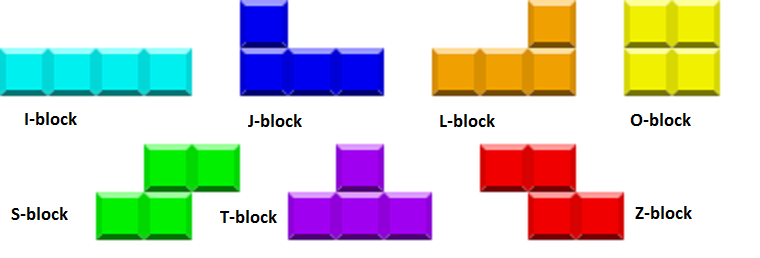
\includegraphics[scale=0.5]{resources/img/tetraminoes}
	\label{tetraminoes}
	}

\section{Spawn Position for Each Tetramino}

	\centering
	\begin{minipage}{0.25\textwidth}
		\centering
		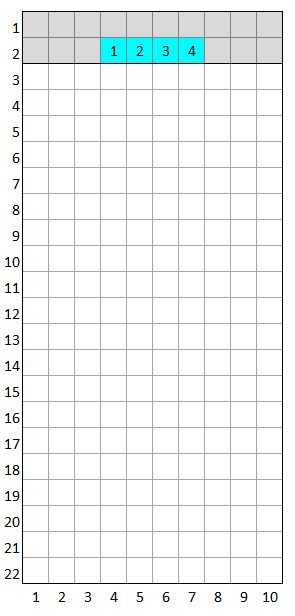
\includegraphics[scale=0.4]{resources/img/minoes/mino_cyan}
		\label{fig:mino-cyan}
	\end{minipage}%
	\begin{minipage}{0.25\textwidth}
		\centering
		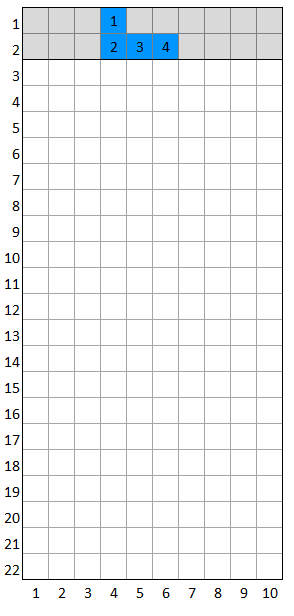
\includegraphics[scale=0.4]{resources/img/minoes/mino_blue}
		\label{fig:mino-blue}
	\end{minipage}%
	\begin{minipage}{0.25\textwidth}
		\centering
		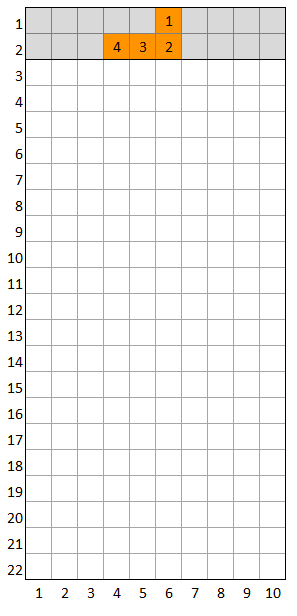
\includegraphics[scale=0.4]{resources/img/minoes/mino_orange}
		\label{fig:mino-orange}
	\end{minipage}%
	\begin{minipage}{0.25\textwidth}
		\centering
		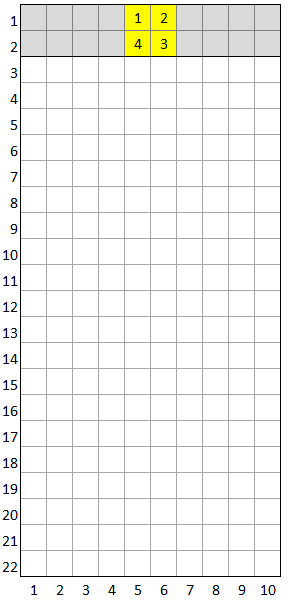
\includegraphics[scale=0.4]{resources/img/minoes/mino_yellow}
		\label{fig:mino-yellow}
	\end{minipage}%
	
	\begin{minipage}{0.33\textwidth}
		\centering
		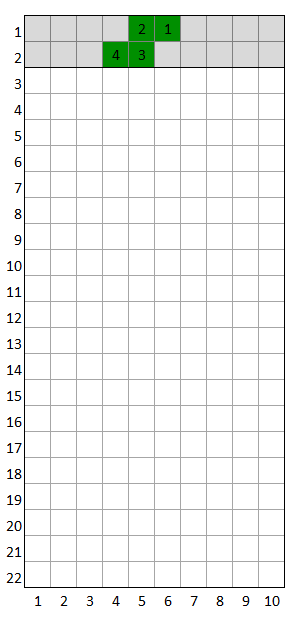
\includegraphics[scale=0.4]{resources/img/minoes/mino_green}
		\label{fig:mino-green}
	\end{minipage}
	\begin{minipage}{0.33\textwidth}
		\centering
		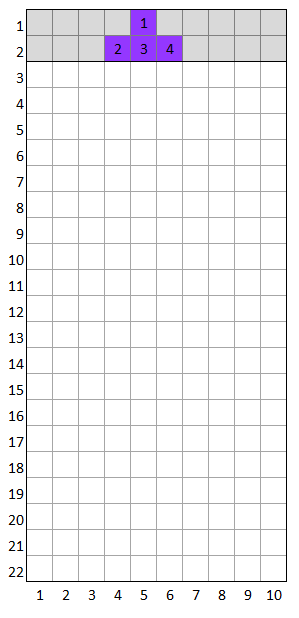
\includegraphics[scale=0.4]{resources/img/minoes/mino_purple}
		\label{fig:mino-purple}
	\end{minipage}%
	\begin{minipage}{0.33\textwidth}
		\centering
		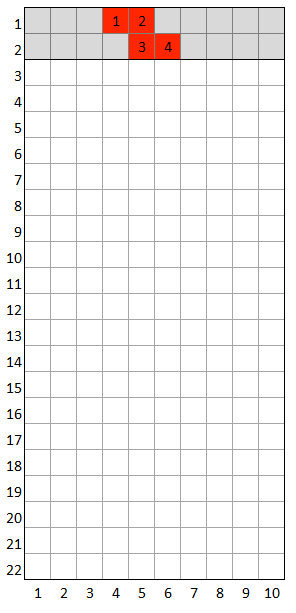
\includegraphics[scale=0.4]{resources/img/minoes/mino_red}
		\label{fig:mino-red}
	\end{minipage}%

Note: The numbers 1, 2, 3 and 4 inside the tetraminoes indicate each mino.

\section{All Possible Orientations of Each Tetramino}
	
	\begin{center}


	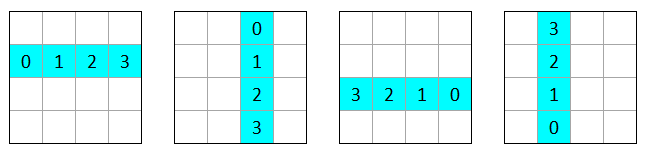
\includegraphics[scale=0.7]{resources/img/orientations/cyan}
	\label{img:cyan}

	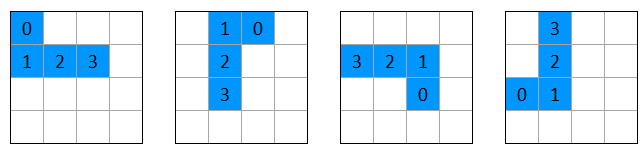
\includegraphics[scale=0.7]{resources/img/orientations/blue}
	\label{img:blue}

	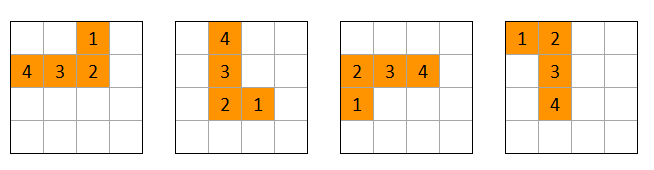
\includegraphics[scale=0.7]{resources/img/orientations/orange}
	\label{img:orange}
	
	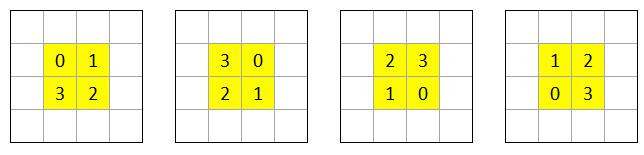
\includegraphics[scale=0.7]{resources/img/orientations/yellow}
	\label{img:yellow}

	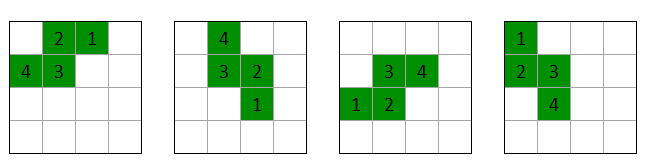
\includegraphics[scale=0.7]{resources/img/orientations/green}
	\label{img:green}

	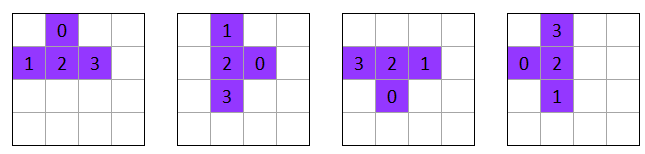
\includegraphics[scale=0.7]{resources/img/orientations/purple}
	\label{img:purple}

	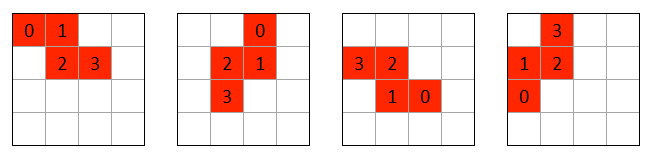
\includegraphics[scale=0.7]{resources/img/orientations/red}
	\label{img:red}

	\end{center}
	
\end{document}
